
\documentclass[11pt]{article}

% ------------------------------------------------------------------------------------------------------------------------
% PACKAGES
% Vous pouvez ajouter des packages si besoin
% Éviter les packages trop exotiques ou connus pour poser des problèmes / incompatibilités
% ------------------------------------------------------------------------------------------------------------------------
\usepackage[utf8]{inputenc}
\usepackage[T1]{fontenc}
\usepackage{siunitx}
\usepackage[dvipsnames]{xcolor}
\sisetup{separate-uncertainty,
locale = FR, scientific-notation = false, exponent-product = \times, inter-unit-product = \ensuremath{{}\cdot{}}}
\usepackage{graphicx}
\usepackage{amsmath, amssymb}
\usepackage[version=4]{mhchem} %affichage des formules chimiques
\usepackage{pgfplots} %plots directement dans latex
\pgfplotsset{height = 7cm,width=12cm,compat=1.9}
% \usepgfplotslibrary{external}
%\tikzexternalize
\usetikzlibrary{angles, arrows.meta, quotes,calc}
\usepackage{float}
\floatplacement{figure}{H}%placement par défaut des figures !h!tbp
\usepackage[%
      a4paper,%
      textwidth=16cm,%
      top=2cm,%
      bottom=2cm,%
      headheight=25pt,%
      headsep=12pt,%
      footskip=25pt]{geometry}%
\usepackage[french]{babel}
\parindent0pt

\usepackage{caption}
\captionsetup{
    labelformat=empty,
    width = .93\textwidth
}

\usepackage{hyperref}

% ------------------------------------------------------------------------------------------------------------------------
% MACROS
% Ne rajouter que des macros réellement nécessaires afin de réduire la probabilité de conflit
% ------------------------------------------------------------------------------------------------------------------------
% Ensembles mathématiques
\def		\K	{	\ensuremath	{\mathbb	{K}	}	}
\def		\N	{	\ensuremath	{\mathbb	{N}	}	}
\def		\NN	{	\ensuremath	{\mathbb	{N}	}	}
\def		\Z	{	\ensuremath	{\mathbb	{Z}	}	}
\def		\Q	{	\ensuremath	{\mathbb	{Q}	}	}
\def		\R	{	\ensuremath	{\mathbb	{R}	}	}
\def		\RR	{	\ensuremath	{\mathbb	{R}	}	}
\def		\C	{	\ensuremath	{\mathbb	{C}	}	}

% Guillemets français et anglais (simples et doubles)
\newcommand{\frquotes}[1]{\og{#1}\fg}
\newcommand{\ensquotes}[1]{`{#1}'}
\newcommand{\enquotes}[1]{``{#1}''}

% Valeurs absolues
\newcommand{\abs}[1]{\ensuremath{\left|{#1}\right|}}

% ------------------------------------------------------------------------------------------------------------------------
% OPÉRATEURS
% ------------------------------------------------------------------------------------------------------------------------
\DeclareMathOperator{\cotan}{cotan}


% ------------------------------------------------------------------------------------------------------------------------
\newcounter{qNum}

\newif\ifdraft
% Le booléen suivant définit si on est en mode draft (avec affichage des réponses vraies/fausses et méta-données) ou production (cases)
% Commenter pour le mode production ; dé-commenter la ligne \draftrue dans le headers.tex pour voir les détails
\drafttrue

\ifdraft
    \newenvironment{question}[4]
    	{\noindent\rule{\textwidth}{0.5pt}\\{\bf Question~:} \refstepcounter{qNum}\theqNum \par{\bf SF~:} #1 \par{\bf Thème~:} #2 \par{\bf Niveau~:} #3 \par{\bf Dépendance~:} #4 \par\noindent\rule{\textwidth}{0.25pt}\\}
    	{ }
    
    \newenvironment{reponses}
    	{\begin{description}}
    	{\end{description}}
\else
    \newenvironment{question}[4]
    	{\refstepcounter{qNum} \subsubsection{ Question \theqNum} \noindent\rule{.5\textwidth}{0.25pt}\\ {\bf SF~:} #1 \par{\bf Thème~:} #2\par{\bf Niveau~:} #3 \par{\bf Dépendance~:} #4 \par \noindent\rule{.5\textwidth}{0.25pt}\\}
    	{ }

    
    \newenvironment{reponses}
    	{\renewcommand{\descriptionlabel}[1]{$\square$} \begin{description}  }
    	{\end{description}}

\fi


\begin{document}
\tableofcontents

\section{Calcul}
	\subsection{Changer d'unité}
		\begin{question}{1215,1214}{Conversions}{1}{}
            L'électronvolt est l'unité commune d'énergie utilisé en physique nucléaire et en atomistique. On définit un électron-volt comme l'énergie cinétique acquise par un électron dans un potentiel de un volt après avoir parcouru \SI{1}{\meter}, soit environ \SI{1.602e-19}{\joule}. La première raie (H$_\alpha$) de l'hydrogène est de longueur d'onde \SI{656.2}{\nano\meter}, ce qui correspond à une énergie de \SI{3.03e-19}{\joule}. À quoi cela correspond-t-il en électronvolts?
        \end{question}
        \begin{reponses}
		    \item[false] Environ \SI{4.856e-38}{\electronvolt}.
		    \item[false] \SI{-13.6}{\electronvolt}
		    \item[true] Environ \SI{1.89}{\electronvolt}.
		    \item[false] Environ \SI{3}{\electronvolt}.
        \end{reponses}
        %%%%%%%%%%%%%%%%%%%%
		
		\begin{question}{}{Conversions}{1}{}
            À combien de \si{\meter} correspond \SI{1}{\angstrom} (\frquotes{un Ångström})?
        \end{question}
        \begin{reponses}
            \item[false] \SI{1e-9}{\meter}
            \item[true] \SI{1e-10}{\meter}
            \item[false] \SI{1e10}{\meter}
            \item[false] \SI{1e-3}{\meter}
        \end{reponses}
        %%%%%%%%%%%%%%%%%%%%
		
		\begin{question}{}{Conversions}{1}{}
			À quoi correspond un \si{ppm} (partie par million)?
        \end{question}
        \begin{reponses} 
            \item[true] \SI{1e-4}{\percent}
            \item[false] \SI{0.01}{\percent}
            \item[true] \num{1e-6}
    	    \item[false] \SI{100}{\percent}
        \end{reponses}
        %%%%%%%%%%%%%%%%%%%%
		\begin{question}{1215,1214}{Conversions}{1}{}
            À combien de \si{\milli\liter} correspond \SI{1}{\centi\meter\cubed}?
        \end{question}
        \begin{reponses}
            \item[false] \SI{10}{\milli\liter}
            \item[false] \SI{1000}{\milli\liter}
            \item[true] \SI{1}{\milli\liter}
            \item[false] \SI{100}{\milli\liter}
        \end{reponses}
        %%%%%%%%%%%%%%%%%%%%
        
        \begin{question}{1215,1214}{Conversions}{1}{}
            À combien de \si{\liter} correspond \SI{1}{\meter\cubed}?
        \end{question}
        \begin{reponses}
            \item[false] \SI{1}{\liter}
            \item[true] \SI{1000}{\liter}
            \item[false] \SI{10}{\liter}
            \item[false] \SI{100}{\liter}
        \end{reponses}
        %%%%%%%%%%%%%%%%%%%%
        
        \begin{question}{}{Conversions}{1}{}
            Quelle est la formule générale de conversion des Kelvin en degrés Celsius?
        \end{question}
        \begin{reponses}
            \item[true] $T[\si{\celsius}] = T[\si{\kelvin}] - \num{273.15}$
            \item[false] $T[\si{\celsius}] = T[\si{\kelvin}] + \num{273.15}$
            \item[false] $T[\si{\kelvin}] = T[\si{\celsius}] - \num{273.15}$
            \item[false] $T[\si{\kelvin}] = T[\si{\celsius}] + \num{273.15}$
        \end{reponses}
        %%%%%%%%%%%%%%%%%%%%
        
        \begin{question}{}{Conversions}{1}{}
            Quelle est la formule générale de conversion des degrés Celsius en Kelvin?
        \end{question}
        \begin{reponses}
            \item[false] $T[\si{\celsius}] = T[\si{\kelvin}] - \num{273.15}$
            \item[false] $T[\si{\celsius}] = T[\si{\kelvin}] + \num{273.15}$
            \item[false] $T[\si{\kelvin}] = T[\si{\celsius}] - \num{273.15}$
            \item[true] $T[\si{\kelvin}] = T[\si{\celsius}] + \num{273.15}$
        \end{reponses}
        %%%%%%%%%%%%%%%%%%%%
        
        \begin{question}{}{Conversions}{2}{}
            Quelles sont les affirmations suivantes vraies?
        \end{question}
        \begin{reponses}
            \item[true] $\SI{1e-9}{\meter} = \SI{1}{\nano\meter}$
            \item[true] $\SI{10e-10}{\meter} = \SI{10}{\angstrom}$
            \item[false] $\SI{1e-3}{\meter} = \SI{3}{\angstrom}$
            \item[false] $\SI{1e-3}{\joule} = \SI{3}{\angstrom}$
        \end{reponses}
        %%%%%%%%%%%%%%%%%%%%
		
		\begin{question}{}{Conversions}{2}{}
            Quelles sont les affirmations suivantes vraies?
        \end{question}
        \begin{reponses}
            \item[true] $\SI{1e-2}{\mole\per\centi\meter\cubed} = \SI{10}{\mole\per\liter}$
            \item[false] $\SI{1}{\milli\mole\per\centi\meter\cubed} = \SI{10}{\mole\per\liter}$
            \item[true] $\SI{1e4}{\mole\per\liter} = \SI{10}{\mole\per\centi\meter\cubed}$
            \item[true] $\SI{0.1}{\milli\mole\per\centi\meter\cubed} = \SI{0.1}{\mole\per\liter}$
        \end{reponses}
        %%%%%%%%%%%%%%%%%%%%
        
        \begin{question}{}{Conversions}{2}{}
            Quelles sont les affirmations suivantes vraies?
        \end{question}
        \begin{reponses}
            \item[true] $\SI{1e-2}{\percent} = \num{1e-4}$
            \item[false] Une atténuation de $3/4$ équivaut à une atténuation de \num{.8}.
            \item[true] $\SI{18}{\percent} = \num{0.18}$
            \item[false] $\SI{18}{\percent} = \num{1.8}$
        \end{reponses}
        %%%%%%%%%%%%%%%%%%%%
        
         \begin{question}{}{Conversions}{2}{}
            Quelles sont les affirmations suivantes vraies?
        \end{question}
        \begin{reponses}
            \item[false] $\SI{2}{\percent} = \num{0.2}$
            \item[true] Une atténuation de $3/4$ équivaut à une amplification de \num{-.75}.
            \item[false] $\SI{3}{\milli\liter} = \num{3e4}$
            \item[true] $\SI{6}{\meter\squared} = \SI{60000}{\centi\meter\squared}$
        \end{reponses}
        %%%%%%%%%%%%%%%%%%%%
    
        \begin{question}{}{Conversions}{2}{}
            Quelles sont les affirmations suivantes vraies?
        \end{question}
        \begin{reponses}
            \item[false] $\SI{0.7}{\percent} = \num{0.07}$
            \item[false] Une atténuation de $4/8$ équivaut à une atténuation de \num{-0.5}.
            \item[true] $\SI{3}{\milli\liter} = \SI{3e3}{\milli\meter\cubed}$
            \item[true] $\SI{6}{\meter\squared} = \SI{6e-6}{\kilo\meter\squared}$
        \end{reponses}
        %%%%%%%%%%%%%%%%%%%%
    
        \begin{question}{}{Conversions}{3}{}
            Quelles sont les affirmations suivantes vraies? On rappelle que $\mathcal{N_A} = \SI{6.02e23}{\per\mole}$.
        \end{question}
        \begin{reponses}
            \item[true] Trois tours par minute équivalent à \SI{0.314}{\radian\per\second}.
            \item[true] $\SI{1}{\mole\per\liter} = \SI{1}{\milli\mole\per\centi\meter\cubed}$
            \item[false] Pour un élément de masse molaire $M = \SI{5}{\gram\per\mole}$: $\SI{3}{\mole\per\liter} = \SI{15}{\gram\per\meter\cubed}$.
            \item[false] $\SI{50}{\kilo\mole\per\meter\cubed} \SI{3e20}{\milli\mole\per\centi\meter\cubed}$
        \end{reponses}
        %%%%%%%%%%%%%%%%%%%%
		
		\begin{question}{}{Conversions}{3}{}
            Quelles sont les affirmations suivantes vraies?
        \end{question}
        \begin{reponses}
            \item[true] $\SI{1e-9}{\meter\cubed} = \SI{1}{\micro\liter}$
            \item[false] $\SI{3e-30}{\liter} = \SI{3}{\angstrom\cubed}$
            \item[true] $\SI{10}{\liter} = \SI{1e-3}{\meter\cubed}$
            \item[false] $\SI{1e-3}{\meter\cubed} = \SI{3}{\angstrom}$
        \end{reponses}
        %%%%%%%%%%%%%%%%%%%%
        
        \begin{question}{}{Conversions}{3}{}
            Quelles sont les affirmations suivantes vraies?
        \end{question}
        \begin{reponses}
            \item[true] $\SI{70}{\kelvin} = \SI{-203.15}{\celsius}$
            \item[false] $\SI{373.15}{\celsius} = \SI{100}{\kelvin}$
            \item[true] $\SI{4}{\kelvin\squared} \simeq \SI{7.24e4}{\celsius\squared}$
            \item[true] $\SI{300}{\kelvin} \simeq \SI{20}{\celsius}$
        \end{reponses}
        %%%%%%%%%%%%%%%%%%%%
		
    
    \subsection{Dans les situations de proportionnalité, trouver une valeur manquante en utilisant une règle de 3}
		\subsubsection{Dilution}
			\begin{question}{}{Dilution}{1}{}
				Lors d'une dilution, quelle est la formule liant la concentration des solutions mère et fille ($C_{m,f}$) aux volumes de dilution et prélevé de la solution mère ($V_{f,m}$)?
			\end{question}
			\begin{reponses}
				\item[true] $C_f\cdot V_f = C_m\cdot V_m$
				\item[false] $C_f\cdot V_m = C_m\cdot V_f$
				\item[false] $C_f/V_f = C_m/V_m$
				\item[false] $V_f/C_f = V_m/C_m$
			\end{reponses}
			%%%%%%%%%%%%%%%%%%%%
		
			\begin{question}{1215,1209,1210,1211}{Dilution}{2}{}
				Lors d'une dilution, les concentrations et volumes des solutions mères et filles sont reliés par $C_f\cdot V_f = C_m\cdot V_m$. Quelle est la concentration d'une solution de la solution fille après dilution par un facteur 100 (c'est à dire que $V_f/V_m = 100$) de la solution mère de HCl à $C_m = \SI{5e2}{\mole\per\liter}$?
			\end{question}
			\begin{reponses}
				\item[false] $C_f = \SI{500}{\mole\per\liter}$
				\item[false] $C_f = \SI{5e4}{\mole\per\liter}$
				\item[true] $C_f = \SI{5}{\mole\per\liter}$
				\item[true] $C_f = \SI{5e3}{\milli\mole\per\liter}$
			\end{reponses}
			%%%%%%%%%%%%%%%%%%%%
			
			\begin{question}{1215,1209}{Dilution}{2}{}
				Lors d'une dilution, les concentrations et volumes des solutions mères et filles sont reliés par $C_f[\si{\mole\per\liter}]\cdot V_f[\si{\liter}] = C_m[\si{\mole\per\liter}]\cdot V_m[\si{\liter}]$. On souhaite diluer une solution d'acide fluorhydrique à $C_m = \SI{.5}{\mole\per\liter}$ pour obtenir une solution \emph{trois fois moins concentrée}. Quel est le facteur de dilution (ratio $V_f/V_m$) que l'on doit appliquer pour réaliser cette opération?
			\end{question}
			\begin{reponses}
				\item[true] $V_f/V_m = \num{3}$
				\item[false] $V_f/V_m = \num{0.3}$
				\item[false] $V_f/V_m = 1/3$
				\item[false] $V_f/V_m = \SI{3}{\liter}$
			\end{reponses}
			%%%%%%%%%%%%%%%%%%%%
		
			\begin{question}{1215,1209,1214,1210,1211}{dilution}{3}{}
				Lors d'une dilution, les concentrations et volumes des solutions mères et filles sont reliés par $C_f\cdot V_f = C_m\cdot V_m$. La législation en matière de stockage du mystérieux agent X a changé, la concentration maximale autorisée dans une solution est désormais de \SI{1}{\mol\per\liter} contre \SI{1}{\kilo\mol\per\liter} auparavant. On dispose d'un volume de \SI{1}{\meter\cubed} qu'il nous faut diluer au plus vite sous peines de poursuites judiciaires. Quelle quantité de liquide obtiendrons-nous après cette dilution? Cela rentre-t-il dans les \emph{quatre cuves de \SI{18000}{\liter}} dont nous disposons?
			\end{question}
			\begin{reponses} 
				\item[true] \SI{1e3}{\meter\cubed}
				\item[false] \SI{10}{\meter\cubed}
				\item[true] Non.
				\item[false] Oui.
			\end{reponses}
			%%%%%%%%%%%%%%%%%%%%
			
			\begin{question}{1215,1209,1214,1210,1211}{Dilution}{3}{}
				Lors d'une dilution, les concentrations et volumes des solutions mères et filles sont reliés par $C_f\cdot V_f = C_m\cdot V_m$. On souhaite diluer une solution d'acide ascorbique à $C_m = \SI{5e2}{\milli\mole\per\liter}$ pour obtenir une solution \emph{dix fois moins concentrée}. Cependant, le récipient dont on dispose pour effectuer cette dilution n'est que de $\SI{50}{\centi\liter}$. Quel volume de la solution initiale doit-on prélever? On ne prend pas en compte le fait que le récipient ne peut se remplir à raz bord en pratique et on considère avoir assez de solution mère à disposition.
			\end{question}
			\begin{reponses} 
				\item[true] \SI{5}{\centi\liter}
				\item[false] On ne peut pas.
				\item[false] \SI{5}{\centi\meter\cubed}
				\item[false] \SI{5}{\milli\liter}
			\end{reponses}
			%%%%%%%%%%%%%%%%%%%%
			
			\begin{question}{1215,1209,1214,1210,1211}{Dilution}{3}{}
				Lors d'une dilution, les concentrations et volumes des solutions mères et filles sont reliés par $C_f\cdot V_f = C_m\cdot V_m$. On souhaite diluer une solution d'acide ascorbique à $C_m = \SI{5e2}{\milli\mole\per\liter}$ pour obtenir une solution dont la concentration est de $C_f = \SI{3}{\milli\mole\per\liter}$. Cependant, le récipient dont on dispose pour effectuer cette dilution n'est que de $\SI{50}{\centi\liter}$. Quel volume de la solution initiale doit-on prélever? On ne prend pas en compte le fait que le récipient ne peut se remplir à raz bord en pratique et on considère avoir assez de solution mère à disposition.
			\end{question}
			\begin{reponses} 
				\item[false] \SI{5}{\micro\liter}
				\item[false] On ne peut pas.
				\item[true] \SI{3}{\centi\meter\cubed}
				\item[true] \SI{3}{\milli\liter}
			\end{reponses}
			%%%%%%%%%%%%%%%%%%%%
			\begin{question}{1215,1209,1214,1210,1211}{Dilution}{3}{}
			Un cafetier italien immigré aux États-Unis doit adapter sa boisson au goût local. Les \textit{ristretto} italiens sont typiquement d'un volume de \SI{2}{\centi\liter}. Les consommateurs américains, quant-à eux apprécient les cafés plus allongés servis dans un gobelet en carton de \SI{50}{\centi\liter}. Ces mêmes clients apprécient également un café moins fort, c'est pourquoi notre cafetier décide d'utiliser la même quantité de café pour les deux préparations (on peut donc considérer que la quantité de matière dissoute dans les deux boissons est la même). Quelle est alors la concentration relative de l'\textit{americano} par rapport à celle du \textit{ristretto}, $C_a/C_r$?
			\end{question}
			\begin{reponses} 
				\item[true] \SI{4}{\percent}
				\item[false] \SI{0.04}{\percent}
				\item[false] \SI{2500}{\percent}
					\item[false] \SI{100}{\percent}
			\end{reponses}
			%%%%%%%%%%%%%%%%%%%%
		
			\begin{question}{1215,1209,1214,1210,1211}{Homéopathie 1}{3}{}
				L'Oscillococcinum, \frquotes{médicament} homéopathique des laboratoires Boiron est fabriqué à partir d'extraits de foie et de c\oe{}ur de canard de Barbarie à \SI{200}{K}. Un \si{K} pour \textit{dynamisation de Korsakov}, correspond à \textit{grosso modo} une dilution au centième de la préparation originale suivie d'une étape appelée dynamisation (agitation de la solution). Quel est le ratio de la concentration mère par rapport à la solution fille après l'élaboration du soit disant médicament?
			\end{question}
			\begin{reponses} 
				\item[true] $C_f/C_m = \num{e-400}$
				\item[false] $C_f/C_m = \num{e200}$
				\item[false] $C_f/C_m = \num{e-100}$
				\item[false] $C_f/C_m = \num{e-200}$
			\end{reponses}
			%%%%%%%%%%%%%%%%%%%%
			
			\begin{question}{1215,1209,1214,1210,1211}{Homéopathie 2}{3}{}
				La solution constitué des abats de canard servant à la préparation d'Oscillococcinum est au départ concentrée à \SI{50}{\gram\per\liter} (\SI{35}{\gram} de foie et \SI{15}{\gram} de c\oe{}ur pour une préparation de \SI{1}{\liter}). Quelle est alors la masse d'abats de canard contenue dans \emph{une unique bille} de lactose (le médicament final) sachant qu'on dispose sur l'ensemble des granules d'un tube (soit 200 granules de \SI{5}{\milli\gram}), \SI{0.01}{\milli\liter} de la solution diluée à \SI{200}{K} (ce qui correspond à $C_f/C_m = \num{e-400}$). À titre informatif, la masse d'un atome de carbone, principal constituant de la matière \frquotes{vivante}, est \SI{2e-26}{\kilo\gram} environ.
			\end{question}
			\begin{reponses} 
				\item[true] \SI{2.5e-406}{\gram\per granule}
				\item[false] \SI{2.6e-7}{\gram\per granule}
				\item[false] \SI{5e-399}{\gram\per granule}
				\item[false] \SI{5e-404}{\gram\per granule}
			\end{reponses}
			%%%%%%%%%%%%%%%%%%%%
			
    \subsection{Remplacer les valeurs littérales par les grandeurs numériques pour calculer une application numérique}
		\begin{question}{}{Formules}{1}{}
			Comment calculer l'erreur sur la mesure de l'énergie d'un photon $E=\hbar\omega$? On notera l'erreur sur la mesure de la pulsation du photon $\delta\omega$ et l'erreur sur la constante de Planck réduite $\delta\hbar$.
        \end{question}
        \begin{reponses}
    	    \item[false] $\delta E = \abs{\frac{\partial E}{\partial \hbar}}\delta \hbar+\abs{\frac{\partial E}{\partial \omega}}\delta \omega$
		    \item[true] $\delta E = \sqrt{\abs{\frac{\partial E}{\partial \hbar}\delta \hbar}^2+\abs{\frac{\partial E}{\partial \omega}\delta \omega}^2}$
		    \item[false] $\delta E = \sqrt{\abs{\frac{\partial E}{\partial \hbar}\delta \hbar}^2-\abs{\frac{\partial E}{\partial \omega}\delta \omega}^2}$
		    \item[false] $\delta E = \sqrt{\frac{\partial E}{\partial \hbar}\delta \hbar^2+\frac{\partial E}{\partial \omega}\delta \omega^2}$
        \end{reponses}
        %%%%%%%%%%%%%%%%%%%%
        
        \begin{question}{1209}{Formules}{2}{}
			Une définition simplifiée du pH est: $\text{pH} = -\log_{10}\left(\text{[H\textsuperscript{+}]}\right)$, avec la concentration donnée en \si{\mol\per\liter}. Quelle est la concentration en ion H\textsuperscript{+} d'une solution de pH de 8? Est-elle acide ou basique?
        \end{question}
        \begin{reponses}
    	    \item[false] $\text{[H\textsuperscript{+}]} = \SI{1.13}{\mol\per\liter}$ et la solution est basique.
    	    \item[true] $\text{[H\textsuperscript{+}]} = \SI{1.0e-8}{\mol\per\liter}$ et la solution est basique.
    	    \item[false] $\text{[H\textsuperscript{+}]} = \SI{1.0e-8}{\mol\per\liter}$ et la solution est acide.
    	    \item[false] $\text{[H\textsuperscript{+}]} = \SI{2}{\mol\per\liter}$ et la solution est acide.
        \end{reponses}
        %%%%%%%%%%%%%%%%%%%%
        
        \begin{question}{1209}{Formules}{2}{}
			Une définition simplifiée du pH est: $\text{pH} = -\log_{10}\left(\text{[H\textsuperscript{+}]}\right)$, avec la concentration donnée en \si{\mol\per\liter}. Quelle est la concentration en ion H\textsuperscript{+} d'une solution de pH de 7? Est-elle acide ou basique?
        \end{question}
        \begin{reponses}
    	    \item[false] $\text{[H\textsuperscript{+}]} = \SI{2}{\mol\per\liter}$ et la solution est basique.
    	    \item[false] $\text{[H\textsuperscript{+}]} = \SI{e-7}{\mol\per\liter}$ et la solution est acide.
    	    \item[true] $\text{[H\textsuperscript{+}]} = \SI{0.1}{\micro\mol\per\liter}$ et la solution est neutre.
    	    \item[false] $\text{[H\textsuperscript{+}]} = \SI{2}{\mol\per\liter}$ et la solution est acide.
        \end{reponses}
        %%%%%%%%%%%%%%%%%%%%
        
        \begin{question}{1209,1210}{pH}{2}{}
			On donne les constantes $K_1 = 1000$, $K_2 = \num{1e14}$ et $K_3 = K_1/K_2$. On définit le pK comme $\text{pK} = -\log_{10}\left(K\right)$. Que vaut pK\textsubscript{3}?
        \end{question}
        \begin{reponses}
    	    \item[true] $\text{pK}_3 = 11$
    	    \item[false] $\text{pK}_3 = 1000$
    	    \item[false] $\text{pK}_3 = \num{1e-11}$
    	    \item[false] $\text{pK}_3 = 0$
        \end{reponses}
        %%%%%%%%%%%%%%%%%%%%
        
        \begin{question}{1209,1210}{pH}{2}{}
			On donne les constantes $K_1 = 1000$, $K_2 = 3$ et $K_3 = K_1^{K_2}$. On définit le pK comme $\text{pK} = -\log_{10}\left(K\right)$. Que vaut pK\textsubscript{3}?
        \end{question}
        \begin{reponses}
    	    \item[false] $\text{pK}_3 = 10$    
    	    \item[true] $\text{pK}_3 = -9$
    	    \item[false] $\text{pK}_3 = \num{1e9}$
    	    \item[false] $\text{pK}_3 = 0$
        \end{reponses}
        %%%%%%%%%%%%%%%%%%%%
        
        \begin{question}{1209,1210}{pH}{2}{}
			On donne les constantes $K_1 = 1000$, $K_2 = 3$ et $K_3 = K_1^{-K_2}$. On définit le pK comme $\text{pK} = -\log_{10}\left(K\right)$. Que vaut pK\textsubscript{3}?
        \end{question}
        \begin{reponses}
    	    \item[false] $\text{pK}_3 = 5$    
    	    \item[false] $\text{pK}_3 = -9$
    	    \item[false] $\text{pK}_3 = \num{1e-9}$
    	    \item[false] $\text{pK}_3 = 0$
        \end{reponses}
        %%%%%%%%%%%%%%%%%%%%
        
        \begin{question}{1210,1211}{Formules}{2}{}
			Le moment dipolaire d'un système de deux charges est le produit de la distance entre les deux charge multiplié par la valeur de la charge positive du système. Les atomes d'hydrogène et de fluor de l'acide fluorhydrique sont séparés d'une distance de \SI{0.92}{\angstrom}. Sachant que la charge positive du système est de $e\,\si{\coulomb}$, quel est le \emph{moment dipolaire} du système?
        \end{question}
        \begin{reponses}
    	    \item[true] $\mu = \SI{1.47e-29}{\coulomb\meter}$
    	    \item[false] $\mu = \SI{0.92}{\coulomb\meter}$
    	    \item[false] $\mu = \SI{1.47e-28}{\coulomb\meter}$
    	    \item[false] $\mu = \SI{0.92e-30}{\coulomb\meter}$
        \end{reponses}
        %%%%%%%%%%%%%%%%%%%%
		
		\begin{question}{1209}{Formules}{2}{}
			Une définition simplifiée du pH est: $\text{pH} = -\log_{10}\left(\text{[H\textsuperscript{+}]}\right)$, avec la concentration donnée en \si{\mol\per\liter}. Quel est le pH d'une solution dont la concentration en ion H\textsuperscript{+} est de \SI{0.1}{\milli\mol\per\liter}? Est-elle acide ou basique?
        \end{question}
        \begin{reponses}
    	    \item[false] Le pH est de \num{4} et la solution est basique.
    	    \item[true] Le pH est d'environ \num{4} et la solution est acide.
    	    \item[false] Le pH est d'environ \num{7} et la solution est neutre.
    	    \item[false] Le pH est d'environ \num{7} et la solution est basique.
        \end{reponses}
        %%%%%%%%%%%%%%%%%%%%
		
		\begin{question}{1209}{Formules}{2}{}
            Une définition simplifiée du pH est: $\text{pH} = -\log_{10}\left(\text{[H\textsuperscript{+}]}\right)$, avec la concentration donnée en \si{\mol\per\liter}. Quel est le pH d'une solution dont la concentration en ion H\textsuperscript{+} est de \SI{0.1}{\mol\per\liter}? Est-elle acide ou basique?
        \end{question}
        \begin{reponses}
    	    \item[false] Le pH est de \num{1.69} et la solution est basique.
    	    \item[true] Le pH est d'environ \num{1.7} et la solution est acide.
    	    \item[false] Le pH est d'environ \num{7} et la solution est neutre.
    	    \item[false] Le pH est d'environ \num{9} et la solution est basique.
        \end{reponses}
        %%%%%%%%%%%%%%%%%%%%
		
		\begin{question}{1209}{Formules}{2}{}
            Une définition simplifiée du pH est: $\text{pH} = -\log_{10}\left(\text{[H\textsuperscript{+}]}\right)$, avec la concentration donnée en \si{\mol\per\liter}. Quelle est la concentration en ion H\textsuperscript{+} d'une solution de pH de -9? Est-elle acide ou basique?
        \end{question}
        \begin{reponses}
    	    \item[false] $\text{[H\textsuperscript{+}]} = \SI{9}{\mol\per\liter}$ et la solution est basique.
    	    \item[false] On ne peut pas savoir.
    	    \item[false] $\text{[H\textsuperscript{+}]} = \SI{1}{\giga\mol\per\liter}$ et la solution est basique.
    	    \item[false] $\text{[H\textsuperscript{+}]} = \SI{1e-9}{\mol\per\liter}$ et la solution est neutre.
        \end{reponses}
        %%%%%%%%%%%%%%%%%%%%
		
		\begin{question}{1209}{Formules}{2}{}
            Une définition simplifiée du pH est: $\text{pH} = -\log_{10}\left(\text{[H\textsuperscript{+}]}\right)$, avec la concentration donnée en \si{\mol\per\liter}. Quelle est la concentration en ion H\textsuperscript{+} d'une solution de pH de 9? Est-elle acide ou basique?
        \end{question}
        \begin{reponses}
    	    \item[false] $\text{[H\textsuperscript{+}]} = \SI{9}{\mol\per\liter}$ et la solution est basique.
    	    \item[true] $\text{[H\textsuperscript{+}]} = \SI{1e-9}{\mol\per\liter}$ et la solution est basique.
    	    \item[true] $\text{[H\textsuperscript{+}]} = \SI{1}{\nano\mol\per\liter}$ et la solution est basique.
    	    \item[false] $\text{[H\textsuperscript{+}]} = \SI{2}{\mol\per\liter}$ et la solution est neutre.
        \end{reponses}
        %%%%%%%%%%%%%%%%%%%%
        
        \begin{question}{1209}{Formules}{2}{}
			Une définition simplifiée du pH est: $\text{pH} = -\log_{10}\left(\text{[H\textsuperscript{+}]}\right)$, avec la concentration donnée en \si{\mol\per\liter}. Quelle est la concentration en ion H\textsuperscript{+} d'une solution de pH de 20? Est-elle acide ou basique?
        \end{question}
        \begin{reponses}
    	    \item[false] $\text{[H\textsuperscript{+}]} = \SI{9}{\mol\per\liter}$ et la solution est basique.
    	    \item[false] $\text{[H\textsuperscript{+}]} = \SI{1e-20}{\mol\per\liter}$ et la solution est basique.
    	    \item[false] $\text{[H\textsuperscript{+}]} = \SI{1}{\nano\mol\per\liter}$ et la solution est basique.
    	    \item[false] $\text{[H\textsuperscript{+}]} = \SI{2}{\mol\per\liter}$ et la solution est neutre.
        \end{reponses}
        %%%%%%%%%%%%%%%%%%%%
        
        \begin{question}{1209,1210}{pH}{2}{}
			On donne les constantes $K_1 = 1000$, $K_2 = \num{1e-2}$ et $K_3 = K_1\times K_2$. On définit le pK comme $\text{pK} = -\log_{10}\left(K\right)$. Que vaut pK\textsubscript{3}?
        \end{question}
        \begin{reponses}
    	    \item[false] $\text{pK}_3 = 100$
    	    \item[false] $\text{pK}_3 = \num{-1e-4}$
    	    \item[true] $\text{pK}_3 = -1$
    	    \item[false] $\text{pK}_3 = 0$
        \end{reponses}
        %%%%%%%%%%%%%%%%%%%%
		
		\begin{question}{1210,1211}{Formules}{2}{}
            L'énergie $E$ d'un photon est donnée par la relation: $E=hc/\lambda$, où $c$ est la célérité de la lumière en \si{\meter\per\second}, $\lambda$ est la longueur d'onde en \si{\meter} et $h$ est la constante de Planck en \si{\joule\second}. Dans quel cas la relation $E=h\nu$ est également juste?
        \end{question}
        \begin{reponses}
            \item[false] $\nu$ est la vitesse du son en \si{\meter\per\second}.
            \item[false] $\nu$ est la longueur d'onde en \si{\nano\meter}.
            \item[true] $\nu$ est la fréquence de la lumière en \si{\per\second}.
            \item[false] $\nu$ est la période de la lumière en \si{\second}.
        \end{reponses}
        %%%%%%%%%%%%%%%%%%%%
		
		\begin{question}{1210,1214,1215}{Formules}{2}{}
			Le Debye noté \si{D} est une unité de mesure du moment dipolaire, $\SI{1}{D} = \SI{3.34e-30}{\coulomb\meter}$. Quelles sont les conversions ci-après justes?
        \end{question}
        \begin{reponses}
    	    \item[true] $\SI{3}{D} \simeq  \SI{1.0e-29}{\coulomb\meter}$
    	    \item[true] $\SI{9e29}{D} \simeq  \SI{3}{\coulomb\meter}$
    	    \item[true] $\SI{1e-4}{D} \simeq  \SI{3.3e-34}{\coulomb\meter}$
    	    \item[true] $\SI{6e14}{D} \simeq  \SI{2.0e-19}{\coulomb\meter}$
        \end{reponses}
        %%%%%%%%%%%%%%%%%%%%
		
		\begin{question}{1210,1211}{Formules}{3}{}
			Les atomes d'hydrogène et de fluor de l'acide fluorhydrique sont séparés d'une distance de \SI{0.92}{\angstrom}. Sachant que la charge positive du système est de $e\,\si{\coulomb}$, quel est le \emph{moment dipolaire} du système?
        \end{question}
        \begin{reponses}
    	    \item[true] $\mu = \SI{1.47e-29}{\coulomb\meter}$
    	    \item[false] $\mu = \SI{0.92}{\coulomb\meter}$
    	    \item[false] $\mu = \SI{1.47e-28}{\coulomb\meter}$
    	    \item[false] $\mu = \SI{0.92e-30}{\coulomb\meter}$
        \end{reponses}
        %%%%%%%%%%%%%%%%%%%%
        
        \begin{question}{1210,1211}{Formules}{3}{}
            Les atomes d'hydrogène et de chlore de l'acide chlorhydrique sont séparés d'une distance de \SI{1.27e-10}{\meter}. Sachant que la charge positive du système est de $e\,\si{\coulomb}$ (la charge de l'électron), quel est le \emph{moment dipolaire} du système?
        \end{question}
        \begin{reponses}
    	    \item[true] $\mu = \SI{2.03e-29}{\coulomb\meter}$
    	    \item[false] $\mu = \SI{1.27}{\coulomb\meter}$
    	    \item[false] $\mu = \SI{2.03e-28}{\coulomb\meter}$
    	    \item[false] $\mu = \SI{1.27e-30}{\coulomb\meter}$
        \end{reponses}
        %%%%%%%%%%%%%%%%%%%%
        
        \begin{question}{1210,1211}{Formules}{3}{}
            Les atomes d'hydrogène et de brome du bromure d'hydrogène sont séparés d'une distance de \SI{0.141}{\nano\meter}. Sachant que la charge positive du système est de $e\,\si{\coulomb}$ (la charge de l'électron), quel est le \emph{moment dipolaire} du système?
        \end{question}
        \begin{reponses}
    	    \item[true] $\mu = \SI{2.26e-29}{\coulomb\meter}$
    	    \item[false] $\mu = \SI{1.41}{\coulomb\meter}$
    	    \item[false] $\mu = \SI{1.58e-28}{\coulomb\meter}$
    	    \item[false] $\mu = \SI{3.40e-30}{\coulomb\meter}$
        \end{reponses}
        %%%%%%%%%%%%%%%%%%%%
        
        \begin{question}{1210,1211}{Formules}{3}{}
			Les atomes d'hydrogène et de chlore de la molécule de iodure d'hydrogène sont séparés d'une distance de \SI{1.61e-10}{\meter}. Sachant que la charge positive du système est de $e\,\si{\coulomb}$ (la charge de l'électron), quel est le \emph{moment dipolaire} du système?
        \end{question}
        \begin{reponses}
    	    \item[true] $\mu = \SI{2.57e-29}{\coulomb\meter}$
    	    \item[false] $\mu = \SI{1.61}{\coulomb\meter}$
    	    \item[false] $\mu = \SI{2.03e-28}{\coulomb\meter}$
    	    \item[false] $\mu = \SI{1.27e-30}{\coulomb\meter}$
        \end{reponses}
        %%%%%%%%%%%%%%%%%%%%
        
    \subsection{Équilibrer une réaction -- Résoudre des équations du premier ordre}
		\begin{question}{8}{Équations}{2}{}
            Quelles sont les valeurs des coefficients de st\oe{}chiométrie $a$ et $b$ de la réaction chimique \ce{CH4 + a\,O2 -> CO2 + b\,H2O}?
        \end{question}
        \begin{reponses}
            \item[false] $a=1$ et $b=2$.
            \item[false] $a=2$ et $b=1$.
            \item[false] $a=4$ et $b=3$.
            \item[true] $a=2$ et $b=2$.
        \end{reponses}
        %%%%%%%%%%%%%%%%%%%%
        
        \begin{question}{8}{Équations}{2}{}
            Quelles sont les valeurs des coefficients de st\oe{}chiométrie $a$, $b$ et $c$ de la réaction chimique \ce{a\,H2 + b\,O2 -> c\,H2O}?
        \end{question}
        \begin{reponses}
            \item[false] $a=1$, $b=2$ et $c=1$.
            \item[true] $a=2$, $b=1$ et $c=2$.
            \item[false] $a=4$, $b=0$ et $c=3$.
            \item[false] $a=2$, $b=2$ et $c=2$.
        \end{reponses}
        %%%%%%%%%%%%%%%%%%%%
		
		\begin{question}{8}{Équations}{2}{}
			Quelles sont les valeurs des coefficients de st\oe{}chiométrie $a$, $b$ et $c$ de la réaction chimique \ce{a\,N2 + b\,H2 -> c\,NH3}?
		\end{question}
		\begin{reponses}
			\item[false] $a=0$, $b=3$ et $c=1$.
			\item[true] $a=1$, $b=3$ et $c=2$.
			\item[false] $a=4$, $b=3$ et $c=3$.
			\item[false] $a=2$, $b=2$ et $c=2$.
		\end{reponses}
		%%%%%%%%%%%%%%%%%%%%
		
		\begin{question}{1216,8,1209}{Calcul de concentration}{2}{}
            L'air est composé majoritairement de di-azote (\emph{deux} atomes d'azote), de di-oxygène (\emph{deux} atomes d'oxygène) et d'\emph{un pourcent} de gaz rares (majoritairement de l'argon). La masse molaire de l'air est de \SI{28.965}{\gram\per\mol}. Quelle est la proportion des différentes espèces dans ce mélange, sachant que la masse molaire de l'azote est \SI{14.007}{\gram\per\mol}, celle de l'oxygène est \SI{15.999}{\gram\per\mol} et celle de l'argon \SI{39.948}{\gram\per\mol}? Rappelez-vous que la somme des proportions des différentes espèces est de \SI{100}{\percent}, c'est à dire que $1 = x_{\ce{N}} + x_{\ce{O}} + x_{\ce{Ar}}$ où $x_i$ désigne la proportion de l'élément en question.
        \end{question}
        \begin{reponses}
            \item[false] \SI{80.112}{\percent} d'azote, \SI{19.365}{\percent} d'oxygène et \SI{0.952}{\percent} d'argon.
		    \item[true] \SI{78.125}{\percent} d'azote, \SI{20.875}{\percent} d'oxygène et \SI{1}{\percent} d'argon.
		    \item[false] On ne peut pas le calculer.
		    \item[false] \SI{79.103}{\percent} d'azote, \SI{19.897}{\percent} d'oxygène et \SI{1}{\percent} d'argon.
        \end{reponses}
        %%%%%%%%%%%%%%%%%%%%
		
		\begin{question}{1216,8,1209}{Calcul de concentration}{3}{}
            L'air est composé majoritairement de di-azote, de di-oxygène et d'\emph{un pourcent} de gaz rares (majoritairement de l'argon). La masse molaire de l'air est de \SI{28.965}{\gram\per\mol}. Quelle est la proportion des différentes espèces dans ce mélange, sachant que la masse molaire de l'azote est \SI{14.007}{\gram\per\mol}, celle de l'oxygène est \SI{15.999}{\gram\per\mol} et celle de l'argon \SI{39.948}{\gram\per\mol}?
        \end{question}
        \begin{reponses}
            \item[false] \SI{80.112}{\percent} d'azote, \SI{19.365}{\percent} d'oxygène et \SI{0.952}{\percent} d'argon.
		    \item[true] \SI{78.125}{\percent} d'azote, \SI{20.875}{\percent} d'oxygène et \SI{1}{\percent} d'argon.
		    \item[false] On ne peut pas le calculer.
		    \item[false] \SI{79.103}{\percent} d'azote, \SI{19.897}{\percent} d'oxygène et \SI{1}{\percent} d'argon.
        \end{reponses}
        %%%%%%%%%%%%%%%%%%%%
		
		\begin{question}{1216,8,1209}{Calcul de concentration}{3}{}
            L'air est composé majoritairement de \SI{78.125}{\percent} de di-azote, de di-oxygène et d'\emph{un pourcent} de gaz rares (majoritairement de l'argon). La masse molaire de ces composants est respectivement de \SI{14.007}{\gram\per\mol}, \SI{15.999}{\gram\per\mol} et \SI{39.948}{\gram\per\mol}. Quelle est la masse molaire de l'air?
        \end{question}
        \begin{reponses}
            \item[false] \SI{40.140}{\gram\per\mol}
		    \item[true] \SI{28.965}{\gram\per\mol}
		    \item[false] On ne peut pas la calculer.
		    \item[false] \SI{34.605}{\gram\per\mol}
        \end{reponses}
        %%%%%%%%%%%%%%%%%%%
    
    \subsection{Passer d'une échelle à une autre}
        \subsubsection{Échelle linéaire à linéaire}
			\begin{question}{8,1219}{Transformation d'échelle}{2}{}
				Quelle est la formule générale permettant de passer de l'échelle du haut (abscisse $x$) à l'échelle du bas (abscisse $y$)? Par exemple, l'étoile rouge a pour coordonnées: $x=\num{-9.5}$ ou $y=\num{-11.5}$. Puisque les échelles sont linéaires, on cherche une relation du type $y = ax+b$ avec $a,b\in\R$.
				\begin{figure}
					\centering
					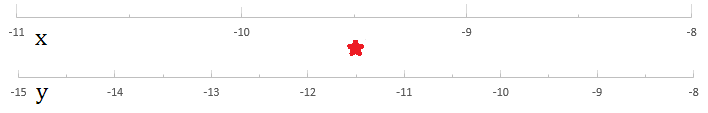
\includegraphics[scale=.75]{Antoine/Figures_Antoine/lin_-11_-8_to_lin_-15_-8_star_-9d5_-11d5.png}
				\end{figure}
			\end{question}
			\begin{reponses}
				\item[true] $y = 7(x+8)/3-8$
				\item[false] $y = 7(x-8)/3+8$
				\item[false] $y = 7x/3-8$
				\item[false] $y = 8/3-8x+7$
			\end{reponses}
			%%%%%%%%%%%%%%%%%%%%
		
			\begin{question}{8,1219}{Transformation d'échelle}{2}{}
				Quelle est la formule générale permettant de passer de l'échelle du haut (abscisse $x$) à l'échelle du bas (abscisse $y$)? Par exemple, l'étoile rouge a pour coordonnées: $x=\num{-9.5}$ ou $y=\num{7.5}$. Puisque les échelles sont linéaires, on cherche une relation du type $y = ax+b$ avec $a,b\in\R$.
				\begin{figure}
					\centering
					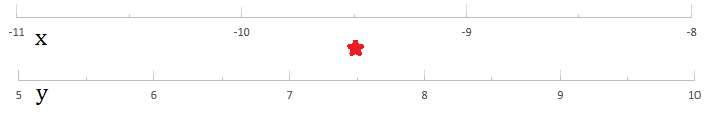
\includegraphics[scale=.75]{Antoine/Figures_Antoine/lin_-11_-8_to_lin_5_10_star_-9d5_7d5.png}
				\end{figure}
			\end{question}
			\begin{reponses}
				\item[true] $y = 5/3\times x+70/3$
				\item[true] $y = 5(x+14)/3$
				\item[false] $y = 3(x+70)/5$
				\item[false] $y = 3x/5+70$
			\end{reponses}
			%%%%%%%%%%%%%%%%%%%%
			
			\begin{question}{8,1219}{Transformation d'échelle}{2}{}
				Quelle est la formule générale permettant de passer de l'échelle du haut (abscisse $x$) à l'échelle du bas (abscisse $y$)? Par exemple, l'étoile rouge a pour coordonnées: $x=3$ ou $y=\num{14}$.
				\begin{figure}
					\centering
					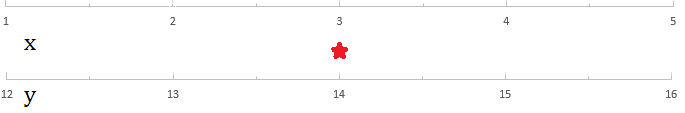
\includegraphics[scale=.75]{Antoine/Figures_Antoine/lin_1_5_to_lin_12_16_star_3_14.png}
				\end{figure}
			\end{question}
			\begin{reponses}
				\item[true] $y = x + 11$
				\item[false] $y = 14/3\times x+12$
				\item[false] $y = 12x-1$
				\item[false] $y = x + 12$
			\end{reponses}
			%%%%%%%%%%%%%%%%%%%%
			
			\begin{question}{8,1219}{Transformation d'échelle}{2}{}
				Quelle est la formule générale permettant de passer de l'échelle du haut (abscisse $x$) à l'échelle du bas (abscisse $y$)? Par exemple, l'étoile rouge a pour coordonnées: $x=5$ ou $y=\num{7.5}$. Puisque les échelles sont linéaires, on cherche une relation du type $y = ax+b$ avec $a,b\in\R$.
				\begin{figure}
					\centering
					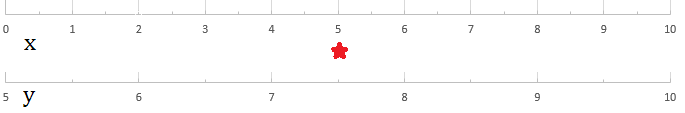
\includegraphics[scale=.75]{Antoine/Figures_Antoine/lin_0_10_to_lin_5_10_star_5_7d5.png}
				\end{figure}
			\end{question}
			\begin{reponses}
				\item[false] $y = 3x$
					\item[false] $y = 1/3\times x+5$
					\item[false] $y = 2 x-5$
					\item[true] $y = \num{0.5}x + 5$
			\end{reponses}
			%%%%%%%%%%%%%%%%%%%%
			
			\begin{question}{8,1219}{Transformation d'échelle}{3}{}
				Quelle est la formule générale permettant de passer de l'échelle du haut (abscisse $x$) à l'échelle du bas (abscisse $y$)? Par exemple, l'étoile rouge a pour coordonnées: $x=5$ ou $y=\num{14}$.
				\begin{figure}
					\centering
    	            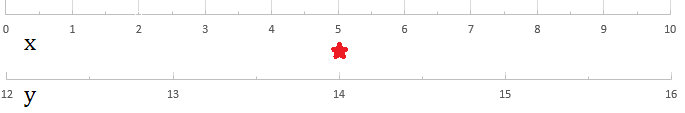
\includegraphics[scale=.75]{Antoine/Figures_Antoine/lin_0_10_to_lin_12_16_star_5_14.png}
				\end{figure}
			\end{question}
			\begin{reponses}
				\item[false] $y = 7x+0$
				\item[true] $y = 2/5\times x+12$
				\item[false] $y = \num{2.5}\times x-12$
				\item[false] $y = \num{5}x + 14$
			\end{reponses}
			%%%%%%%%%%%%%%%%%%%%
			
        \subsubsection{Échelle linéaire à logarithmique}
			\begin{question}{8,1219,1211,1222,1227}{Transformation d'échelle}{2}{}
				Quelle est la formule générale permettant de passer de l'échelle du haut (abscisse $x$) à l'échelle du bas (abscisse $y$)? Par exemple, l'étoile rouge a pour coordonnées: $x=\num{3}$ ou $y\simeq\num{2}$. Puisque l'on passe d'une échelle linéaire à une échelle logarithmique, on cherche une relation du type $y = a10^{bx}$ avec $a,b\in\R$.
				\begin{figure}
					\centering
					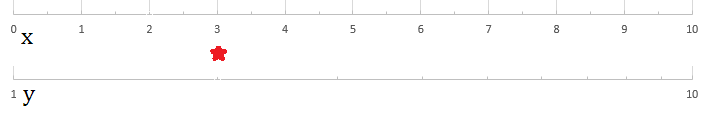
\includegraphics[scale=.75]{Antoine/Figures_Antoine/lin_1_10_to_log_1_10_star_3_2.png}
				\end{figure}
			\end{question}
			\begin{reponses}
				\item[false] $y = 10^{10x+1}$
				\item[false] $y = 10^{10x}$
				\item[true] $y = 10^{\num{.1}x}$
				\item[false] $y = 10\times 10^{10x}$
			\end{reponses}
			%%%%%%%%%%%%%%%%%%%%
		
			\begin{question}{8,1219,1211,1222,1227}{Transformation d'échelle}{2}{}
				Quelle est la formule générale permettant de passer de l'échelle du haut (abscisse $x$) à l'échelle du bas (abscisse $y$)? Par exemple, l'étoile rouge a pour coordonnées: $x=\num{1000}$ ou $y=\num{-12}$. Puisque l'on passe d'une échelle logarithmique à une échelle linéaire, on cherche une relation du type $y = a\log_{10}(bx)$ avec $a,b\in\R$.
				\begin{figure}
					\centering
					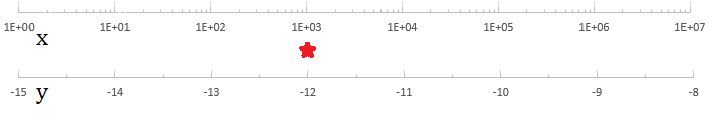
\includegraphics[scale=.75]{Antoine/Figures_Antoine/log_1_1e7_to_lin_-15_-8_star_1e3_-12.png}
				\end{figure}
			\end{question}
			\begin{reponses}
				\item[false] $y = 5\log_{10}(2x)$
				\item[false] $y = -15\log_{10}(10x)$
				\item[true] $y = -15+\log_{10}(x)$
				\item[false] $20\log_{10}(x)$
			\end{reponses}
			%%%%%%%%%%%%%%%%%%%%
		
        \subsubsection{Échelle logarithmique à logarithmique}
			\begin{question}{8,1219,1211,1222,1227}{Transformation d'échelle}{3}{}
				Quelle est la formule générale permettant de passer de l'échelle du haut (abscisse $x$) à l'échelle du bas (abscisse $y$)? Par exemple, l'étoile rouge a pour coordonnées: $x=\num{1e3}$ ou $y\simeq\num{2683}$. Puisque l'on passe d'une échelle logarithmique à une échelle logarithmique, on cherche une relation du type $y = a\log_{10}(bx)$ avec $a,b\in\R$.
				\begin{figure}
					\centering
					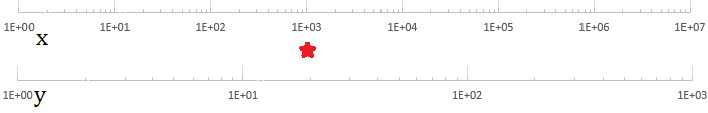
\includegraphics[scale=.75]{Antoine/Figures_Antoine/log_1_1e7_to_log_1_1e3_star_1e3_2e1.png}
				\end{figure}
			\end{question}
			\begin{reponses}
				\item[true] $y = x^{8/7}$
				\item[false] $y = 7/8\log_{10}(x)$
				\item[false] $y = x^{\num{7/8}}$
				\item[false] $\log_{10}(y) = \num{7}\log_{10}(x) + 8$
			\end{reponses}
			%%%%%%%%%%%%%%%%%%%%
			\begin{question}{8,1219,1211,1222,1227}{Transformation d'échelle}{3}{}
				Quelle est la formule générale permettant de passer de l'échelle du haut (abscisse $x$) à l'échelle du bas (abscisse $y$)? Par exemple, l'étoile rouge a pour coordonnées: $x=\num{4}$ ou $y=\num{2}$. Puisque l'on passe d'une échelle logarithmique à une échelle logarithmique, on cherche une relation du type $\log_{10}(y) = a\log_{10}(bx)$ avec $a,b\in\R$. Attention à bien faire le calcul, la réponse n'est peut-être pas si évidente (pensez à utiliser les propriétés des logarithmes et puissances).
				\begin{figure}
					\centering
					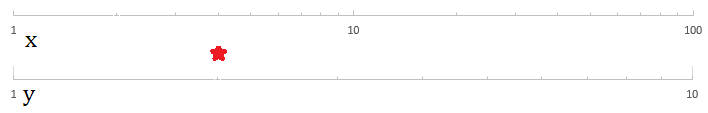
\includegraphics[scale=.75]{Antoine/Figures_Antoine/log_1_100_to_log_1_10_star_4_2.png}
				\end{figure}
			\end{question}
			\begin{reponses}
				\item[false] $y = \num{0.5}\log_{10}(x)$
					\item[false] $y = x^2+\num{0.5}$
					\item[false] $y = \num{10}\log_{10}(x) + 5$
					\item[true] $y = x^{\num{0.5}}$
			\end{reponses}
			%%%%%%%%%%%%%%%%%%%%
    
    %ajouter idées de MJ ramage (voir correction) + Loreynne
    %ajouter avec réaction https://www.techniques-ingenieur.fr/actualite/articles/8-reactions-chimiques-incroyables-2866/ mesurer la taille de la colonne après la réaction.
    
\section{Modélisation}
%Déterminer le coefficient d'extinction molaire à partir de la représentation graphique de l'absorbance d'une solution en fonction de sa concentration (loi de Beer-lambert).
	\subsection{Reconnaissance de courbe}
		\begin{question}{N.A.}{Reconnaissance de courbes}{1}{}
			Parmi les différentes représentations de la figure suivante, laquelle représente une évolution périodique?
			\begin{figure}
				\centering
				\begin{tikzpicture}
					\begin{axis}[
						title = {Représentations graphiques de différentes quantités},
						axis lines = left,
						xlabel = $x$,
						%minor x tick num = 4,
						ylabel = $y$,
						ymin=0, ymax=40,
						/pgf/number format/.cd,%3 lignes dessous, utiliser spacers français au eu d'anglais.
						use comma,
						1000 sep={\,}
					]
						%Below the red curve
						\addplot [
							domain=0:10,
							samples=100,
							color=red,
							style=dotted,
							%/pgf/text mark = {+}, %changer le marqueur text
							%mark=*,
						]
						{10^(0.2*x)};
						\addplot [
							domain=0:10,
							samples=100,
							color=blue,
							%/pgf/text mark = {+}, %changer le marqueur text
							mark=*,
						]
						{10*sin(100*x)};
						\addplot [
							domain=0:10,
							samples=100,
							color=black,
							style=solid,
							%/pgf/text mark = {+}, %changer le marqueur text
							%mark=o,
						]
						{3*x};
						\addplot [
							domain=0:10,
							samples=100,
							color=green,
							style=dashed,
							%/pgf/text mark = {+}, %changer le marqueur text
							%mark=triangle,
						]
						{3*x^2};
					\end{axis}
				\end{tikzpicture}
			\end{figure}
		\end{question}
		\begin{reponses}
		\item[true] La courbe bleue (cercles).
		\item[false] La courbe rouge (pointillés).
		\item[false] La courbe noire (pleine).
		\item[false] La courbe verte (tirets).
		\end{reponses}
		%%%%%%%%%%%%%%%%%%%%
		\begin{question}{N.A.}{Reconnaissance de courbes}{1}{}
            Parmi les différentes représentations de la figure suivante, laquelle représente une évolution exponentielle?
            \begin{figure}
              \begin{tikzpicture}
                  \begin{semilogyaxis}[
                        title = {Représentations graphiques de différentes quantités},
                        axis lines = left,
                        xlabel = $x$,
                        %minor x tick num = 4,
                        ylabel = $y$,
                        ymax=100,
                        /pgf/number format/.cd,%3 lignes dessous, utiliser spacers français au lieu d'anglais.
                        use comma,
                        1000 sep={\,}
                      ]
                      %Below the red curve
                      \addplot [
                        domain=0:10,
                        samples=100,
                        color=red,
                        style=dotted
                        %/pgf/text mark = {+}, %changer le marqueur text
                        %mark=o,
                      ]
                      {10^(0.2*x)};
                      \addplot [
                        domain=0.0001:10,
                        samples=100,
                        color=blue,
                        %/pgf/text mark = {+}, %changer le marqueur text
                        mark=*,
                      ]
                      {1/(3*x)};
                      \addplot [
                        domain=0:10,
                        samples=100,
                        color=black,
                        style=solid,
                        %/pgf/text mark = {+}, %changer le marqueur text
                        %mark=o,
                      ]
                      {3*x};
                      \addplot [
                        domain=0:10,
                        samples=100,
                        color=green,
                        style=dashed,
                        %/pgf/text mark = {+}, %changer le marqueur text
                        %mark=o,
                      ]
                      {3*x^2};
                  \end{semilogyaxis}
              \end{tikzpicture}
             \end{figure}
        \end{question}
        \begin{reponses}
            \item[false] La courbe bleue (cercles).
		    \item[true] La courbe rouge (pointillés).
		    \item[false] La courbe noire (pleine).
		    \item[false] La courbe verte (tirets).
		    \end{reponses}
        %%%%%%%%%%%%%%%%%%%%
        
        \begin{question}{N.A.}{Reconnaissance de courbes}{2}{}
            Parmi les différentes représentations de la figure suivante, laquelle représente une évolution exponentielle?
            \begin{figure}
              \begin{tikzpicture}
                  \begin{semilogyaxis}[
                        title = {Représentations graphiques de différentes quantités},
                        axis lines = left,
                        xlabel = $x$,
                        %minor x tick num = 4,
                        ylabel = $y$,
                        ymax=100,
                        /pgf/number format/.cd,%3 lignes dessous, utiliser spacers français au lieu d'anglais.
                        use comma,
                        1000 sep={\,}
                      ]
                      %Below the red curve
                      \addplot [
                        domain=0:10,
                        samples=100,
                        color=red,
                        style=dotted
                        %/pgf/text mark = {+}, %changer le marqueur text
                        %mark=o,
                      ]
                      {exp(x)};
                      \addplot [
                        domain=0.0001:10,
                        samples=100,
                        color=blue,
                        %/pgf/text mark = {+}, %changer le marqueur text
                        mark=*,
                      ]
                      {1/x};
                      \addplot [
                        domain=0:10,
                        samples=100,
                        color=black,
                        style=solid,
                        %/pgf/text mark = {+}, %changer le marqueur text
                        %mark=o,
                      ]
                      {x};
                      \addplot [
                        domain=0:10,
                        samples=100,
                        color=green,
                        style=dashed,
                        %/pgf/text mark = {+}, %changer le marqueur text
                        %mark=o,
                      ]
                      {x^2};
                  \end{semilogyaxis}
              \end{tikzpicture}
             \end{figure}
        \end{question}
        \begin{reponses}
            \item[false] La courbe bleue (cercles).
		    \item[true] La courbe rouge (pointillés).
		    \item[false] La courbe noire (pleine).
		    \item[false] La courbe verte (tirets).
		    \end{reponses}
        %%%%%%%%%%%%%%%%%%%%
		\begin{question}{N.A.}{Reconnaissance de courbes}{1}{}
            Parmi les différentes représentations de la figure suivante, laquelle représente une évolution exponentielle?
            \begin{figure}
              \begin{tikzpicture}
                  \begin{axis}[
                        title = {Représentations graphiques de différentes quantités},
                        axis lines = left,
                        xlabel = $x$,
                        %minor x tick num = 4,
                        ylabel = $y$,
                        ymin=0, ymax=40,
                        /pgf/number format/.cd,%3 lignes dessous, utiliser spacers français au lieu d'anglais.
                        use comma,
                        1000 sep={\,}
                      ]
                      %Below the red curve
                      \addplot [
                        domain=0:10,
                        samples=100,
                        color=red,
                        style=dotted
                        %/pgf/text mark = {+}, %changer le marqueur text
                        %mark=o,
                      ]
                      {10^(0.2*x)};
                      \addplot [
                        domain=0.0001:10,
                        samples=100,
                        color=blue,
                        mark=*,
                        %/pgf/text mark = {+}, %changer le marqueur text
                      ]
                      {1/(3*x)};
                      \addplot [
                        domain=0:10,
                        samples=100,
                        color=black,
                        %/pgf/text mark = {+}, %changer le marqueur text
                        %mark=o,
                        style=solid,
                      ]
                      {3*x};
                      \addplot [
                        domain=0:10,
                        samples=100,
                        color=green,
                        style=dashed,
                        %/pgf/text mark = {+}, %changer le marqueur text
                        %mark=o,
                      ]
                      {3*x^2};
                  \end{axis}
              \end{tikzpicture}
             \end{figure}
        \end{question}
        \begin{reponses}
            \item[false] La courbe bleue (cercles).
		    \item[true] La courbe rouge (pointillés).
		    \item[false] La courbe noire (pleine).
		    \item[false] La courbe verte (tirets).
		    \end{reponses}
        %%%%%%%%%%%%%%%%%%%%
		
		\begin{question}{N.A.}{Reconnaissance de courbes}{2}{}
            Parmi les différentes représentations de la figure suivante, laquelle représente une évolution linéaire?
            \begin{figure}
              \begin{tikzpicture}
                  \begin{semilogyaxis}[
                        title = {Représentations graphiques de différentes quantités},
                        axis lines = left,
                        xlabel = $x$,
                        %minor x tick num = 4,
                        ylabel = $y$,
                        ymax=100,
                        /pgf/number format/.cd,%3 lignes dessous, utiliser spacers français au lieu d'anglais.
                        use comma,
                        1000 sep={\,}
                      ]
                      %Below the red curve
                      \addplot [
                        domain=0:10,
                        samples=100,
                        color=red,
                        style=dotted
                        %/pgf/text mark = {+}, %changer le marqueur text
                        %mark=o,
                      ]
                      {exp(x)};
                      \addplot [
                        domain=0.0001:10,
                        samples=100,
                        color=blue,
                        %/pgf/text mark = {+}, %changer le marqueur text
                        mark=*,
                      ]
                      {1/x};
                      \addplot [
                        domain=0:10,
                        samples=100,
                        color=black,
                        style=solid,
                        %/pgf/text mark = {+}, %changer le marqueur text
                        %mark=o,
                      ]
                      {x};
                      \addplot [
                        domain=0:10,
                        samples=100,
                        color=green,
                        style=dashed,
                        %/pgf/text mark = {+}, %changer le marqueur text
                        %mark=o,
                      ]
                      {x^2};
                  \end{semilogyaxis}
              \end{tikzpicture}
             \end{figure}
        \end{question}
        \begin{reponses}
            \item[false] La courbe bleue (cercles).
		    \item[false] La courbe rouge (pointillés).
		    \item[true] La courbe noire (pleine).
		    \item[false] La courbe verte (tirets).
		    \end{reponses}
        %%%%%%%%%%%%%%%%%%%%
	
	\subsection{Questions basiques sur des représentations graphiques connues}
		\begin{question}{N.A.}{Représentation graphique}{1}{}
            La représentation d'une fonction périodique diffère-t-elle quand on la représente selon une échelle semi-logarithmique selon l'axe des ordonnées?
        \end{question}
        \begin{reponses}
            \item[false] Non.
		    \item[false] Oui.
		    \item[true] La représentation de la période reste la même mais la représentation des ordonnées change.
		    \item[false] La représentation de la période change mais la représentation des ordonnées reste la même.
	    \end{reponses}
        %%%%%%%%%%%%%%%%%%%%
		
		\begin{question}{27}{Formalisme mathématique}{1}{}
            Considérons les points $A(1,3)$ et $B(7,1)$ de la droite ci-après. Quel est le coefficient directeur de cette droite?
            \begin{figure}
              \begin{tikzpicture}
                  \begin{axis}[
                        axis lines = left,
                        xlabel = $x$,
                        minor x tick num = 4,
                        ylabel = $y$,
                        /pgf/number format/.cd,%3 lignes dessous, utiliser spacers français au lieu d'anglais.
                        use comma,
                        1000 sep={}
                      ]
                      %Below the red curve
                      \addplot [
                        domain=0:10,
                        samples=30,
                        color=black,
                        %/pgf/text mark = {+}, %changer le marqueur text
                        %mark=o,
                      ]
                      {-1/3*x+10/3};
                      \addplot [
                        color=red,
                        mark=*,
                      ]
                      coordinates {(1,3)}
                      node[pin=10:{$A$}]{};
                      \addplot [
                        color=red,
                        mark=*,
                      ]
                      coordinates {(7,1)}
                      node[pin=10:{$B$}]{};
                  \end{axis}
              \end{tikzpicture}
             \end{figure}
        \end{question}
        \begin{reponses}
            \item[false] $-3$
		    \item[true] $-1/3$
		    \item[false] $2/3$
		    \item[false] $3/2$
		    \end{reponses}
        %%%%%%%%%%%%%%%%%%%%
		
        \begin{question}{27}{Formalisme mathématique}{2}{}
           Quel est le coefficient directeur de la droite ci-après?
            \begin{figure}
              \begin{tikzpicture}
                  \begin{axis}[
                        axis lines = left,
                        xlabel = $x$,
                        minor x tick num = 4,
                        ylabel = $y$,
                        /pgf/number format/.cd,%3 lignes dessous, utiliser spacers français au lieu d'anglais.
                        use comma,
                        1000 sep={}
                      ]
                      %Below the red curve
                      \addplot [
                        domain=0:10,
                        samples=30,
                        color=black,
                        style = dashed,
                        %/pgf/text mark = {+}, %changer le marqueur text
                        %mark=o,
                      ]
                      {1/3*x+2};
                  \end{axis}
              \end{tikzpicture}
             \end{figure}
        \end{question}
        \begin{reponses}
            \item[false] $-3$
		    \item[false] $-1/3$
		    \item[true] $1/3$
		    \item[false] $2$
		    \end{reponses}
        %%%%%%%%%%%%%%%%%%%%
        
        \begin{question}{27}{Formalisme mathématique}{2}{}
           Quel est l'ordonnée à l'origine de la droite ci-après?
            \begin{figure}
              \begin{tikzpicture}
                  \begin{axis}[
                        axis lines = left,
                        xlabel = $x$,
                        minor x tick num = 4,
                        ylabel = $y$,
                        /pgf/number format/.cd,%3 lignes dessous, utiliser spacers français au lieu d'anglais.
                        use comma,
                        1000 sep={}
                      ]
                      %Below the red curve
                      \addplot [
                        domain=0:10,
                        samples=30,
                        color=black,
                        style = dashed,
                        %/pgf/text mark = {+}, %changer le marqueur text
                        %mark=o,
                      ]
                      {1/3*x+2};
                  \end{axis}
              \end{tikzpicture}
             \end{figure}
        \end{question}
        \begin{reponses}
            \item[false] $-3$
		    \item[false] $0$
		    \item[false] $1/3$
		    \item[true] $2$
		    \end{reponses}
        %%%%%%%%%%%%%%%%%%%%
		
		\begin{question}{27}{Beer-Lambert}{1}{}
            Considérons la fonction $f(x) = A\cdot 10^{-\alpha x}$ avec $A$ et $\alpha$ des constantes positives. La figure ci-après montre la représentation graphique en échelle semi-logarithmique ($\log_{10}$) de la fonction normalisée $f(x)/A$ pour plusieurs valeurs de $x$. Quelle est la valeur du coefficient $\alpha$?
            \begin{figure}
              \begin{tikzpicture}
                  \begin{axis}[
                        axis lines = left,
                        xlabel = $x$,
                        minor x tick num = 4,
                        ylabel = $f(x)/A$,
                        /pgf/number format/.cd,%3 lignes dessous, utiliser spacers français au lieu d'anglais.
                        use comma,
                        1000 sep={}
                      ]
                      %Below the red curve
                      \addplot [
                        domain=0:20,
                        samples=30,
                        color=red,
                        %/pgf/text mark = {+}, %changer le marqueur text
                        %mark=o,
                      ]
                      {-0.5*x*10};% pour  y = a . exp(-b . x) , - a.b est la pente de la tangente à la courbe en x = 0. Cette droite coupe l'axe X en x = 1/b. Pour un même a, b indique donc la rapidité de la décroissance de la fonction.
                  \end{axis}
              \end{tikzpicture}
             \end{figure}
        \end{question}
        \begin{reponses}
            \item[false] $\alpha = \num{0.5}$
		    \item[true] $\alpha = 5$
		    \item[false] $\alpha = -5$
		    \item[false] $\alpha = \num{0.2}$
		    \end{reponses}
        %%%%%%%%%%%%%%%%%%%%
        
        \begin{question}{27}{Beer-Lambert}{1}{}
            Considérons la fonction $f(x) = A\cdot 10^{-\alpha x}$ avec $A$ et $\alpha$ des constantes positives. La figure ci-après montre la représentation graphique en échelle semi-logarithmique ($\log_{10}$) de la fonction normalisée $f(x)/A$ pour plusieurs valeurs de $x$. Quelle est la valeur du coefficient $A$?
            \begin{figure}
              \begin{tikzpicture}
                  \begin{axis}[
                        axis lines = left,
                        xlabel = $x$,
                        minor x tick num = 4,
                        ylabel = $f(x)/A$,
                        /pgf/number format/.cd,%3 lignes dessous, utiliser spacers français au lieu d'anglais.
                        use comma,
                        1000 sep={}
                      ]
                      %Below the red curve
                      \addplot [
                        domain=0:20,
                        samples=30,
                        color=red,
                        %/pgf/text mark = {+}, %changer le marqueur text
                        %mark=o,
                      ]
                      {x*10};% pour  y = a . exp(-b . x) , - a.b est la pente de la tangente à la courbe en x = 0. Cette droite coupe l'axe X en x = 1/b. Pour un même a, b indique donc la rapidité de la décroissance de la fonction.
                  \end{axis}
              \end{tikzpicture}
             \end{figure}
        \end{question}
        \begin{reponses}
            \item[false] $A = 0$
		    \item[true] On ne peut pas connaître $A$.
		    \item[false] $A = \num{-5}$
		    \item[false] $A = \num{5}$
		    \end{reponses}
        %%%%%%%%%%%%%%%%%%%%
        
        \begin{question}{27}{Beer-Lambert}{1}{}
            Considérons la fonction $f(x) = A\cdot 10^{-\alpha x}$ avec $A$ et $\alpha$ des constantes positives. La figure ci-après montre la représentation graphique en échelle semi-logarithmique ($\log_{10}$) de la fonction normalisée $f(x)/A$ pour plusieurs valeurs de $x$. Que vaut $A$?
            \begin{figure}
              \begin{tikzpicture}
                  \begin{axis}[
                        axis lines = left,
                        xlabel = $x$,
                        minor x tick num = 4,
                        ylabel = $f(x)/A$,
                        /pgf/number format/.cd,%3 lignes dessous, utiliser spacers français au lieu d'anglais.
                        use comma,
                        1000 sep={}
                      ]
                      %Below the red curve
                      \addplot [
                        domain=0:20,
                        samples=30,
                        color=red,
                        %/pgf/text mark = {+}, %changer le marqueur text
                        %mark=o,
                      ]
                      {-0.5*x*10};% pour  y = a . exp(-b . x) , - a.b est la pente de la tangente à la courbe en x = 0. Cette droite coupe l'axe X en x = 1/b. Pour un même a, b indique donc la rapidité de la décroissance de la fonction.
                  \end{axis}
              \end{tikzpicture}
             \end{figure}
        \end{question}
        \begin{reponses}
            \item[false] $A = 1$
		    \item[false] $A = 4$
		    \item[false] $A = \num{0.2}$
		    \item[true] On ne peut pas connaître $A$.
		    \end{reponses}
        %%%%%%%%%%%%%%%%%%%%
		
	
	
	\subsection{Loi de Beer-lambert}
		\begin{question}{27}{Beer-Lambert}{2}{}
            La loi de Beer-Lambert traduit l'absorption de la lumière passant à travers une solution de concentration $C[\si{\mole\per\liter}]$. Il s'agit d'une loi exponentielle définie par $I(l) = I_0\cdot 10^{-\epsilon l C}$ où $I_0$ est l'intensité de la lumière avant la solution et  $l[\si{\centi\meter}]$ la distance dans la solution. $\epsilon$ est appelé le \emph{coefficient d'extinction molaire} et traduit de la capacité d'une mole de liquide à absorber la lumière (à une longueur d'onde donnée en général). À partir des données expérimentales ci-après et sachant que la solution de bromure de potassium est concentrée à \SI{2.5}{\mole\per\liter}, quelle est la valeur de ce coefficient? On rappelle que la tangente à l'origine d'une loi exponentielle $y = A^{-\alpha x}, A = Cste.$ coupe l'axe des abscisses en $x_0 = 1/\alpha$
            \begin{figure}
              \begin{tikzpicture}
                  \begin{axis}[
                        title = {Intensité lumineuse normalisée en fonction de la distance dans la solution},
                        axis lines = left,
                        xlabel = $l$ (\si{\centi\meter}),
                        minor x tick num = 4,
                        ylabel = $I(l)/I_0$,
                        /pgf/number format/.cd,%3 lignes dessous, utiliser spacers français au lieu d'anglais.
                        use comma,
                        1000 sep={\,}
                      ]
                      %Below the red curve
                      \addplot [
                        domain=0:20,
                        samples=30,
                        color=red,
                        %/pgf/text mark = {+}, %changer le marqueur text
                        mark=o,
                      ]
                      {10^(-0.2*x*2.5)};% pour  y = a . exp(-b . x) , - a.b est la pente de la tangente à la courbe en x = 0. Cette droite coupe l'axe X en x = 1/b. Pour un même a, b indique donc la rapidité de la décroissance de la fonction.
                  \end{axis}
              \end{tikzpicture}
             \end{figure}
        \end{question}
        \begin{reponses}
            \item[false] $\epsilon \simeq \SI{2}{\liter\per\mole\per\centi\meter}$
		    \item[true] $\epsilon \simeq \SI{.2}{\liter\per\mole\per\centi\meter}$
		    \item[false] $\epsilon \simeq \SI{1}{\liter\per\mole\per\centi\meter}$
		    \item[false] $\epsilon \simeq \SI{100}{\liter\per\mole\per\centi\meter}$
		    \end{reponses}
        %%%%%%%%%%%%%%%%%%%%
		
        \begin{question}{27}{Beer-Lambert}{2}{}
            Considérons la loi définie par $I(x) = e^{-\alpha x}$. $\alpha$ est alors un coefficient d'extinction. À partir des données ci-après, quelle est la valeur de ce coefficient? On rappelle que la tangente à l'origine d'une loi exponentielle coupe l'axe des abscisses en $x_0 = 1/\alpha$
            \begin{figure}
              \begin{tikzpicture}
                  \begin{axis}[
                        axis lines = left,
                        xlabel = $x$,
                        minor x tick num = 4,
                        ylabel = $I(x)$,
                        /pgf/number format/.cd,%3 lignes dessous, utiliser spacers français au lieu d'anglais.
                        use comma,
                        1000 sep={\,}
                      ]
                      %Below the red curve
                      \addplot [
                        domain=0:8,
                        samples=30,
                        color=red,
                        %/pgf/text mark = {+}, %changer le marqueur text
                        mark=o,
                      ]
                      {e^(-.5*x)};% pour  y = a . exp(-b . x) , - a.b est la pente de la tangente à la courbe en x = 0. Cette droite coupe l'axe X en x = 1/b. Pour un même a, b indique donc la rapidité de la décroissance de la fonction.
                  \end{axis}
              \end{tikzpicture}
             \end{figure}
        \end{question}
        \begin{reponses}
            \item[false] $\alpha \simeq \num{5}$
		    \item[true] $\alpha \simeq \num{0.5}$
		    \item[false] $\alpha \simeq \num{1}$
		    \item[false] $\alpha \simeq \num{2}$
		    \end{reponses}
        %%%%%%%%%%%%%%%%%%%%
        
        \begin{question}{27}{Beer-Lambert}{3}{}
            La loi de Beer-Lambert traduit l'absorption de la lumière passant à travers une solution de concentration $C[\si{\mole\per\liter}]$. Il s'agit d'une loi exponentielle définie par $I(l) = I_0\cdot 10^{-\epsilon l C}$ où $I_0$ est l'intensité de la lumière avant la solution et  $l[\si{\centi\meter}]$ la distance dans la solution. $\epsilon$ est appelé le \emph{coefficient d'extinction molaire} et traduit de la capacité d'une mole de liquide à absorber la lumière (à une longueur d'onde donnée en général). À partir des données expérimentales ci-après et sachant que la solution de chlorure de potassium est concentrée à \SI{10}{\mole\per\liter}, quelle est la valeur de ce coefficient?
            \begin{figure}
              \begin{tikzpicture}
                  \begin{axis}[
                        title = {Intensité lumineuse normalisée en fonction de la distance dans la solution},
                        axis lines = left,
                        xlabel = $l$ (\si{\centi\meter}),
                        minor x tick num = 4,
                        ylabel = $\log_{10}\left(I(l)/I_0\right)$,
                        /pgf/number format/.cd,%3 lignes dessous, utiliser spacers français au lieu d'anglais.
                        use comma,
                        1000 sep={}
                      ]
                      %Below the red curve
                      \addplot [
                        domain=0:20,
                        samples=30,
                        color=red,
                        %/pgf/text mark = {+}, %changer le marqueur text
                        mark=o,
                      ]
                      {-0.5*x*10};% pour  y = a . exp(-b . x) , - a.b est la pente de la tangente à la courbe en x = 0. Cette droite coupe l'axe X en x = 1/b. Pour un même a, b indique donc la rapidité de la décroissance de la fonction.
                  \end{axis}
              \end{tikzpicture}
             \end{figure}
        \end{question}
        \begin{reponses}
            \item[false] $\epsilon \simeq \SI{5}{\liter\per\mole\per\centi\meter}$
		    \item[true] $\epsilon \simeq \SI{.5}{\liter\per\mole\per\centi\meter}$
		    \item[false] $\epsilon \simeq \SI{1}{\liter\per\mole\per\centi\meter}$
		    \item[false] $\epsilon \simeq \SI{100}{\liter\per\mole\per\centi\meter}$
	    \end{reponses}
        %%%%%%%%%%%%%%%%%%%%
		
		\begin{question}{27}{Beer-Lambert}{3}{}
            La loi de Beer-Lambert traduit l'absorption de la lumière passant à travers une solution de concentration $C[\si{\mole\per\liter}]$. Il s'agit d'une loi exponentielle définie par $I(l) = I_0\cdot 10^{-\epsilon l C}$ où $I_0$ est l'intensité de la lumière avant la solution et  $l[\si{\centi\meter}]$ la distance dans la solution. $\epsilon$ est appelé le \emph{coefficient d'extinction molaire} et traduit de la capacité d'une mole de liquide à absorber la lumière (à une longueur d'onde donnée en général). À partir des données expérimentales ci-après et sachant que la solution de chlorure de sodium est concentrée à \SI{6}{\mole\per\liter}, quelle est la valeur de ce coefficient? Quelle est l'intensité initiale de la lumière incidente?
        \begin{figure}
            \begin{tikzpicture}
                \begin{axis}[
                        title = {Intensité lumineuse normalisée en fonction de la distance dans la solution},
                        axis lines = left,
                        xlabel = $l$ (\si{\centi\meter}),
                        minor x tick num = 4,
                        ylabel = $I(l)$ (\si{{u.a.}}),
                        /pgf/number format/.cd,%3 lignes dessous, utiliser spacers français au lieu d'anglais.
                        use comma,
                        1000 sep={}
                        ]
                    %Below the red curve
                    \addplot[
                        domain=0:10,
                        samples=30,
                        color=red,
                        %/pgf/text mark = {+}, %changer le marqueur text
                        mark=o,
                        ]
                    {30*10^(-0.07*x*6)};% pour  y = a . exp(-b . x) , - a.b est la pente de la tangente à la courbe en x = 0. Cette droite coupe l'axe X en x = 1/b. Pour un même a, b indique donc la rapidité de la décroissance de la fonction.
                \end{axis}
              \end{tikzpicture}
             \end{figure}
        \end{question}
        \begin{reponses}
            \item[false] $\epsilon \simeq \SI{6}{\liter\per\mole\per\centi\meter}$
		    \item[true] $\epsilon \simeq \SI{.07}{\liter\per\mole\per\centi\meter}$
		    \item[true] $I_0 = \SI{30}{{u.a.}}$
		    \item[false] $I_0 = \SI{16}{{u.a.}}$
	    \end{reponses}
        %%%%%%%%%%%%%%%%%%%%
		
		\begin{question}{27}{Beer-Lambert}{3}{}
            La loi de Beer-Lambert traduit l'absorption de la lumière passant à travers une solution de concentration $C[\si{\mole\per\liter}]$. Il s'agit d'une loi exponentielle définie par $I(l) = I_0\cdot 10^{-\epsilon l C}$ où $I_0$ est l'intensité de la lumière avant la solution et  $l[\si{\centi\meter}]$ la distance dans la solution. $\epsilon$ est appelé le \emph{coefficient d'extinction molaire} et traduit de la capacité d'une mole de liquide à absorber la lumière (à une longueur d'onde donnée en général). À partir des données expérimentales ci-après et sachant que la solution de chlorure de potassium est concentrée à \SI{10}{\mole\per\liter}, quelle est la valeur de ce coefficient?
            \begin{figure}
              \begin{tikzpicture}
                  \begin{axis}[
                        title = {Intensité lumineuse normalisée en fonction de la distance dans la solution},
                        axis lines = left,
                        xlabel = $l$ (\si{\centi\meter}),
                        minor x tick num = 4,
                        ylabel = $\log_{10}\left(I(l)/I_0\right)$,
                        /pgf/number format/.cd,%3 lignes dessous, utiliser spacers français au lieu d'anglais.
                        use comma,
                        1000 sep={}
                      ]
                      %Below the red curve
                      \addplot [
                        domain=0:20,
                        samples=30,
                        color=red,
                        %/pgf/text mark = {+}, %changer le marqueur text
                        mark=o,
                      ]
                      {-0.5*x*10};% pour  y = a . exp(-b . x) , - a.b est la pente de la tangente à la courbe en x = 0. Cette droite coupe l'axe X en x = 1/b. Pour un même a, b indique donc la rapidité de la décroissance de la fonction.
                  \end{axis}
              \end{tikzpicture}
             \end{figure}
        \end{question}
        \begin{reponses}
            \item[false] $\epsilon \simeq \SI{5}{\liter\per\mole\per\centi\meter}$
		    \item[true] $\epsilon \simeq \SI{.5}{\liter\per\mole\per\centi\meter}$
		    \item[false] $\epsilon \simeq \SI{1}{\liter\per\mole\per\centi\meter}$
		    \item[false] $\epsilon \simeq \SI{100}{\liter\per\mole\per\centi\meter}$
	    \end{reponses}
        %%%%%%%%%%%%%%%%%%%%
		
    \subsection{Représentation de molécules}
		\begin{question}{N.A.}{Structure de molécules}{1}{}
			Quelle est la structure moléculaire de la molécule de \ce{H2O} dont une représentation est donnée ci-après?
			\begin{figure}
				\centering
				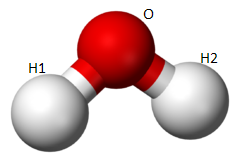
\includegraphics[height = 5cm]{Antoine/Figures_Antoine/240px-Water-3D-balls.png}
			\end{figure}
		\end{question}
		\begin{reponses}
			\item[false] Tétraédrique.
			\item[false] Cristalline cubique.
			\item[false] Linéaire.
			\item[true] En coude.
		\end{reponses}
		%%%%%%%%%%%%%%%%%%%%
		
		\begin{question}{N.A.}{Structure de molécules}{1}{}
			Quand on regarde par le dessus (selon la flèche rouge) une molécule d'eau \ce{H2O} dont une représentation est donnée ci-après, quelle figure observera-t-on?
			\begin{figure}
				\centering
				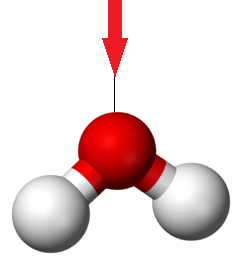
\includegraphics[height = 5cm]{Antoine/Figures_Antoine/240px-Water-3D-balls3.png}
			\end{figure}
		\end{question}
		\begin{reponses}
			\item[false] Un triangle dont les sommets sont les ombres des atomes composant la molécule.
			\item[true] Trois taches alignées formées par les ombres des atomes d'hydrogène, d'oxygène et d'hydrogène.
			\item[false] Un triangle équilatéral formé par l'ombre des trois atomes composant la molécules.
		\end{reponses}
		%%%%%%%%%%%%%%%%%%%%
		
		\begin{question}{N.A.}{Structure de molécules}{1}{}
			Quelle est la structure moléculaire de la molécule de \ce{CH4} dont une représentation est donnée ci-après?
			\begin{figure}
				\centering
				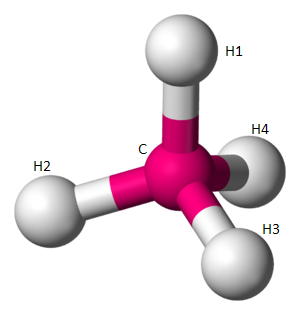
\includegraphics[height = 5cm]{Antoine/Figures_Antoine/300px-Tetrahedral-3D-balls.png}
			\end{figure}
		\end{question}
		\begin{reponses}
			\item[true] Tétraédrique.
			\item[false] Cristalline cubique.
			\item[false] Linéaire.
			\item[false] En diamant.
		\end{reponses}
		%%%%%%%%%%%%%%%%%%%%
		
		\begin{question}{N.A.}{Structure de molécules}{2}{}
			La molécule d'eau forme un coude au niveau de l'atome d'oxygène. L'angle $\widehat{\ce{H}_1\ce{O}\ce{H}_2}$ \SI{105}{\degree}. Quelle est alors la valeur de l'angle formé par l'atome d'oxygène et les atomes d'hydrogène (angle $\widehat{\ce{O}\ce{H}_1\ce{H}_2}$)?
			\begin{figure}
				\centering
				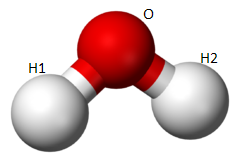
\includegraphics[height = 5cm]{Antoine/Figures_Antoine/240px-Water-3D-balls.png}
			\end{figure}
		\end{question}
		\begin{reponses}
			\item[true] \SI{37.5}{\degree}
				\item[false] \SI{45}{\degree}
				\item[false] \SI{105.5}{\degree}
				\item[false] \SI{20}{\degree}
		\end{reponses}
		%%%%%%%%%%%%%%%%%%%%
		
		\begin{question}{N.A.}{Structure de molécules}{2}{}
			La molécule \ce{CH4} forme un tétrahèdre dont l'atome de carbone est le centre. \SI{109}{\degree}. L'angle $\widehat{\ce{H}_1\ce{C}\ce{H}_2}$ vaut \SI{109}{\degree}. Que vaut alors l'angle $\widehat{\ce{C}\ce{H}_1\ce{H}_2}$?
			\begin{figure}
				\centering
				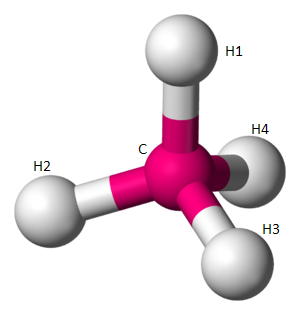
\includegraphics[height = 5cm]{Antoine/Figures_Antoine/300px-Tetrahedral-3D-balls.png}
			\end{figure}
		\end{question}
		\begin{reponses}
			\item[true] \SI{35.5}{\degree}
			\item[false] \SI{45}{\degree}
			\item[false] \SI{30.3}{\degree}
			\item[false] \SI{20.4}{\degree}
		\end{reponses}
		%%%%%%%%%%%%%%%%%%%%
		
		\begin{question}{N.A.}{Structure de molécules}{2}{}
			La molécule d'eau forme un coude dont l'atome d'oxygène est le centre. L'angle $\widehat{\ce{O}\ce{H}_1\ce{H}_2}$ vaut \SI{37.5}{\degree}. Quelle est alors la valeur de l'angle formé $\widehat{\ce{H}_1\ce{O}\ce{H}_2}$?
			\begin{figure}
				\centering
				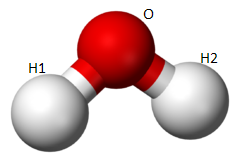
\includegraphics[height = 4cm]{Antoine/Figures_Antoine/240px-Water-3D-balls.png}
			\end{figure}
		\end{question}
			\begin{reponses}
			\item[true] \SI{105}{\degree}
			\item[false] \SI{45}{\degree}
			\item[false] \SI{100}{\degree}
			\item[false] \SI{20}{\degree}
			\end{reponses}
		%%%%%%%%%%%%%%%%%%%%
		
    \subsection{Représentation de structures cristallines}
        \begin{question}{31}{Structures cristallines}{2}{}
            La structure cristalline du tungstène est du type \emph{cubique centré} comme montré par le schéma ci-dessous. Quelle est la valeur de l'angle indiqué par un arc de cercle rouge en fonction de $a$, le paramètre de maille? (indice: faites des dessins des différentes vues).
            \begin{figure}
                \centering
                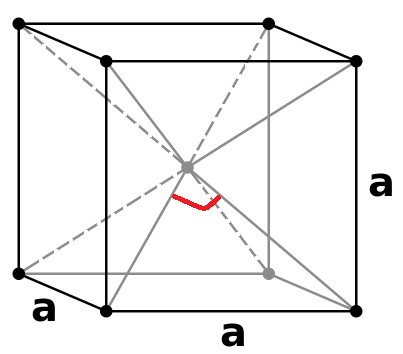
\includegraphics[height = 4cm]{Antoine/Figures_Antoine/BCC2.png}
                \caption{Schéma d'une structure cubique centrée. Les atomes sont matérialisés par les points de jonction du cube. L'atome central se trouve au centre de la structure.}
            \end{figure}
        \end{question}
        \begin{reponses} 
            \item[true] \SI{90}{\degree}
            \item[false] \SI{45}{\degree} 
            \item[false] \SI{180}{\degree}
    	    \item[false] \SI{60}{\degree}
        \end{reponses}
        %%%%%%%%%%%%%%%%%%%%
        
        \begin{question}{31}{Structure cristalline}{2}{}
            La structure cristalline de l'or est du type \emph{cubique faces centrées} comme montré par le schéma ci-dessous. Quelle est la valeur de l'angle indiqué par un arc de cercle rouge en fonction de $a$, le paramètre de maille? (indice: faites des dessins des différentes vues).
            \begin{figure}
                \centering
                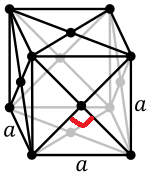
\includegraphics[height = 4cm]{Antoine/Figures_Antoine/FCC2.png}
                \caption{Schéma d'une structure cubique faces centrées. Les atomes sont matérialisés par les points de jonction du cube. Chaque face du cube possède un atome central.}
            \end{figure}
        \end{question}
        \begin{reponses} 
            \item[true] \SI{90}{\degree}
            \item[false] \SI{45}{\degree} 
            \item[false] \SI{180}{\degree}
    	    \item[false] \SI{60}{\degree}
        \end{reponses}
        %%%%%%%%%%%%%%%%%%%%
        
        \begin{question}{31}{Structures cristallines}{3}{}
            La structure cristalline du niobium est du type \emph{cubique centré} comme montré par le schéma ci-dessous. Si on considère que les atomes sont des boules indéformables collées les unes aux autres de rayon $R$, quelle est l'expression du paramètre de maille $a$ en fonction de $R$? (indice: faites des dessins des différentes vues).
            \begin{figure}
                \centering
                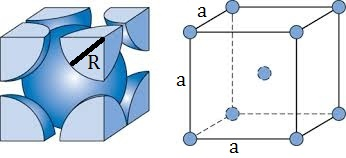
\includegraphics[height = 4cm]{Antoine/Figures_Antoine/BCC.png}
                \caption{Schéma d'une structure cubique centrée. La position des atomes sont matérialisés par les points noirs mais ils se touchent en réalité. L'atome central se trouve au centre de la structure.}
            \end{figure}
        \end{question}
        \begin{reponses} 
            \item[false] $a = 2R$
            \item[false] $a = 4R$
            \item[false] $a = 2R/\sqrt{2}$
    	    \item[true] $a = 4R\sqrt{3}$
        \end{reponses}
        %%%%%%%%%%%%%%%%%%%%
        
        \begin{question}{31}{Structures cristallines}{3}{}
            La structure cristalline du fer est du type \emph{cubique centré} comme montré par le schéma ci-dessous. Si on considère que les atomes sont des boules indéformables collées les unes aux autres de rayon $R$, quelle est l'expression de la compacité $c = \frac{\text{Volume total de la maille}}{\text{Volume occupé par les atomes}}$ en fonction du paramètre de maille $a$ et/ou de $R$? (indice: faites des dessins des différentes vues. Plusieurs réponses sont possibles).
            \begin{figure}
                \centering
                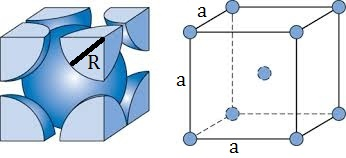
\includegraphics[height = 4cm]{Antoine/Figures_Antoine/BCC.png}
                \caption{Schéma d'une structure cubique centrée. La position des atomes sont matérialisés par les points noirs mais ils se touchent en réalité. L'atome central se trouve au centre de la structure.}
            \end{figure}
        \end{question}
        \begin{reponses} 
            \item[true] $c = \frac{2\times V_\text{atome}}{a^3}$
            \item[false] $c = \frac{9V_\text{atome}}{a^3}$
            \item[true] $c = \frac{8(\pi R^3)}{3a^3}$
    	    \item[false] $c = \frac{3(\pi R^3)}{4a^3}$
        \end{reponses}
        %%%%%%%%%%%%%%%%%%%%
        
        \begin{question}{31}{Structures cristallines}{3}{}
            La structure cristalline du diamant est du type \emph{cubique faces centrées} comme montré par le schéma ci-dessous. Si on considère que les atomes sont des boules indéformables collées les unes aux autres de rayon $R$, quelle est l'expression du paramètre de maille $a$ en fonction de $R$? (indice: faites des dessins des différentes vues).
            \begin{figure}
                \centering
                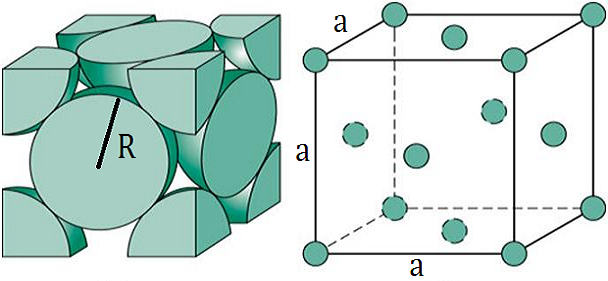
\includegraphics[height = 4cm]{Antoine/Figures_Antoine/FCC.png}
                \caption{Schéma d'une structure cubique faces centrées. La position des atomes sont matérialisés par les points noirs mais ils se touchent en réalité.  Chaque face du cube possède un atome central.}
            \end{figure}
        \end{question}
        \begin{reponses} 
            \item[false] $a = 2R$
            \item[false] $a = 4R$
            \item[false] $a = 2R/\sqrt{3}$
    	    \item[true] $a = 4R\sqrt{2}$
        \end{reponses}
        %%%%%%%%%%%%%%%%%%%%
        
        \begin{question}{31}{Structures cristallines}{3}{}
            La structure cristalline du silicium est du type \emph{cubique faces centrées} comme montré par le schéma ci-dessous. Si on considère que les atomes sont des boules indéformables collées les unes aux autres de rayon $R$, quelle est l'expression de la compacité $c = \frac{\text{Volume total de la maille}}{\text{Volume occupé par les atomes}}$ en fonction du paramètre de maille $a$ et/ou de $R$? (indice: faites des dessins des différentes vues. Plusieurs réponses sont possibles).
            \begin{figure}
                \centering
                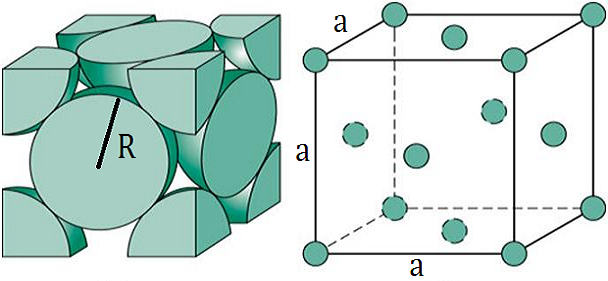
\includegraphics[height = 4cm]{Antoine/Figures_Antoine/FCC.png}
                \caption{Schéma d'une structure cubique faces centrées. La position des atomes sont matérialisés par les points noirs mais ils se touchent en réalité.  Chaque face du cube possède un atome central.}
            \end{figure}
        \end{question}
        \begin{reponses} 
            \item[true] $c = \frac{4\times V_\text{atome}}{a^3}$
            \item[false] $c = \frac{14V_\text{atome}}{a^3}$
            \item[false] $c = \frac{4(\pi R^3)}{3a^3}$
    	    \item[true] $c = \frac{12(\pi R^3)}{4a^3}$
        \end{reponses}
        %%%%%%%%%%%%%%%%%%%%
        
        \begin{question}{31}{Structures cristallines}{3}{}
            La structure cristalline du silicium est du type \emph{cubique faces centrées} comme montré par le schéma ci-dessous. Si on considère que les atomes sont des boules indéformables collées les unes aux autres de rayon $R$. La compacité $c = \frac{\text{Volume total de la maille}}{\text{Volume occupé par les atomes}}$, renseigne sur l'espace libre disponible dans un cristal. Connaître $c$ est utile pour doper le cristal avec d'autres éléments, ce qui est très utile en physique des semi-conducteurs où l'ajout d'autres éléments à un cristal change ses propriétés électriques. Quelle est la valeur de ce paramètre pour cette maille? (indice: faites des dessins des différentes vues).
            \begin{figure}
                \centering
                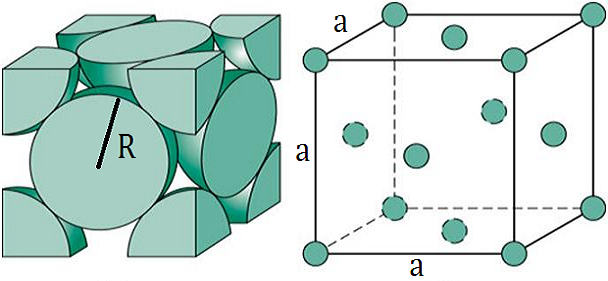
\includegraphics[height = 4cm]{Antoine/Figures_Antoine/FCC.png}
                \caption{Schéma d'une structure cubique faces centrées. La position des atomes sont matérialisés par les points noirs mais ils se touchent en réalité.  Chaque face du cube possède un atome central.}
            \end{figure}
        \end{question}
        \begin{reponses} 
            \item[true] $c = \frac{\pi\sqrt{2}}{6}$
            \item[false] $c = 12$
            \item[false] $c = \frac{3\sqrt{2}}{5}$
    	    \item[false] $c = \num{0.5}$
        \end{reponses}
        %%%%%%%%%%%%%%%%%%%%
        
        \begin{question}{31}{Structures cristallines}{3}{}
            La structure cristalline du fer est du type \emph{cubique centré} comme montré par le schéma ci-dessous. Si on considère que les atomes sont des boules indéformables collées les unes aux autres de rayon $R$. La compacité $c = \frac{\text{Volume total de la maille}}{\text{Volume occupé par les atomes}}$, renseigne sur l'espace libre disponible dans un cristal. Connaître $c$ est utile pour doper le cristal avec d'autres éléments, ce qui est très utile en physique des semi-conducteurs où l'ajout d'autres éléments à un cristal change ses propriétés électriques. Quelle est la valeur de ce paramètre pour cette maille? (indice: faites des dessins des différentes vues).
            \begin{figure}
                \centering
                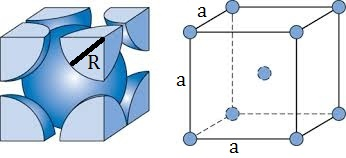
\includegraphics[height = 4cm]{Antoine/Figures_Antoine/BCC.png}
                \caption{Schéma d'une structure cubique centrée. La position des atomes sont matérialisés par les points noirs mais ils se touchent en réalité. L'atome central se trouve au centre de la structure.}
            \end{figure}
        \end{question}
        \begin{reponses} 
            \item[true] $c = \frac{\pi\sqrt{3}}{8}$
            \item[false] $c = \frac{\pi\sqrt{3}}{4}$
            \item[false] $c = \frac{\pi\sqrt{2}}{8}$
    	    \item[false] $c = \num{.5}$
        \end{reponses}
        %%%%%%%%%%%%%%%%%%%%
        
        
        \section{Primitives}
        
        
        \subsection{Intégration graphique}
		\begin{question}{27,1213}{Intégration graphique}{3}{1188}
           La droite ci-après représente l'évolution de la concentration d'azote dissoute dans une solution \emph{à chaque instant}. Quelle est la quantité totale d'azote cumulée entre le début de l'expérience ($t=\SI{0}{\second}$) et la fin au bout d'\emph{une minute}?
            \begin{figure}
              \begin{tikzpicture}
                  \begin{axis}[
                        axis lines = left,
                        xlabel = $t\;(\si{\second})$,
                        %minor x tick num = 4,
                        ylabel = {$[\ce{N}]\;(\si{\mol\per\liter\per\second})$},
                        /pgf/number format/.cd,%3 lignes dessous, utiliser délimitation décimale français au lieu d'anglais.
                        use comma,
                        1000 sep={}
                      ]
                      %Below the red curve
                      \addplot [
                        domain=0:70,
                        samples=2,
                        color=red,
                        %/pgf/text mark = {+}, %changer le marqueur text
                        %mark=o,
                      ]
                      {3};
                  \end{axis}
              \end{tikzpicture}
             \end{figure}
        \end{question}
        \begin{reponses}
            \item[false] \SI{-54}{\mol\per\liter}
		    \item[true] \SI{180}{\mol\per\liter}
		    \item[false] \SI{3}{\mol\per\liter}
		    \item[false] \SI{30}{\mol\per\liter}
		    \end{reponses}
        %%%%%%%%%%%%%%%%%%%%
        
        \begin{question}{27,1213}{Intégration graphique}{3}{1188}
            La droite ci-après représente l'évolution de la concentration \emph{instantanée} d'azote dissoute dans une solution à chaque instant. Quelle est la quantité totale d'azote cumulée entre le début de l'expérience ($t=\SI{0}{\second}$) et la fin au bout de \emph{trente secondes}?
            \begin{figure}
              \begin{tikzpicture}
                  \begin{axis}[
                        axis lines = left,
                        xlabel = $t\;(\si{\second})$,
                        %minor x tick num = 4,
                        ylabel = {$[\ce{N}]\;(\si{\mol\per\liter\per\second})$},
                        /pgf/number format/.cd,%3 lignes dessous, utiliser délimitation décimale français au lieu d'anglais.
                        use comma,
                        1000 sep={}
                      ]
                      %Below the red curve
                      \addplot [
                        domain=0:40,
                        samples=2,
                        color=red,
                        %/pgf/text mark = {+}, %changer le marqueur text
                        %mark=o,
                      ]
                      {x};
                      \addplot [
                        color=red,
                        %mark=*,
                      ]
                      coordinates {(20,20)}
                      node[pin=0:{$y=x$}]{};
                  \end{axis}
              \end{tikzpicture}
             \end{figure}
        \end{question}
        \begin{reponses}
            \item[false] \SI{-14}{\mol\per\liter}
		    \item[true] \SI{450}{\mol\per\liter}
		    \item[false] \SI{900}{\mol\per\liter}
		    \item[false] \SI{30}{\mol\per\liter}
		    \end{reponses}
        %%%%%%%%%%%%%%%%%%%%
        
        \begin{question}{27,1213}{Intégration graphique}{3}{1188}
             Ci-après, on représente l'évolution de la concentration d'oxygène dissoute dans une solution \emph{à chaque instant}. Au bout de trente secondes d'expérience, on éclaire la solution et le phytoplancton présent dans la solution produit de l'oxygène par photosynthèse. Quelle est la quantité totale d'oxygène \emph{cumulée} entre le début de l'expérience ($t=\SI{0}{\second}$) et la fin au bout d'\emph{une minute trente secondes}?
            \begin{figure}
              \begin{tikzpicture}
                  \begin{axis}[
                        axis lines = left,
                        ymin=10,   ymax=90,
                        xlabel = $t\;(\si{\second})$,
                        %minor x tick num = 4,
                        ylabel = {$[\ce{O}]\;(\si{\mol\per\liter\per\second})$},
                        /pgf/number format/.cd,%3 lignes dessous, utiliser délimitation décimale français au lieu d'anglais.
                        use comma,
                        1000 sep={}
                      ]
                      %Below the red curve
                      \addplot [
                        color=red,
                        %/pgf/text mark = {+}, %changer le marqueur text
                        %mark=o,
                      ]
                      coordinates {(0,20) (30,20)};
                      \addplot [
                        domain=30:90,
                        samples=2,
                        color=red,
                        %/pgf/text mark = {+}, %changer le marqueur text
                        %mark=o,
                      ]
                      {(x-30)+20};
                      \addplot [
                       color=red,
                        %mark=*,
                      ]
                      coordinates {(40,30)}
                      node[pin=0:{$y=(x-30)+20$}]{};
                  \end{axis}
              \end{tikzpicture}
             \end{figure}
        \end{question}
        \begin{reponses}
            \item[false] \SI{-10}{\mol\per\liter}
		    \item[true] \SI{3090}{\mol\per\liter}
		    \item[false] \SI{900}{\mol\per\liter}
		    \item[false] \SI{120}{\mol\per\liter}
		\end{reponses}
        %%%%%%%%%%%%%%%%%%%%
		
		\begin{question}{27,1213}{Intégration graphique}{3}{1188}
             Ci-après, on représente l'évolution de la concentration de dioxyde de carbone dissoute dans une solution. Il existe naturellement du \ce{CO2} dissout dans l'eau à une concentration de \SI{20}{\mol\per\liter}. Au bout de trente secondes d'expérience, on éclaire la solution et le phytoplancton présent dans la solution produit de l'oxygène par photosynthèse en transformant le dioxyde de carbone. Quelle est la quantité approximative de \ce{CO2} \emph{cumulée} entre le début de l'expérience ($t=\SI{0}{\second}$) et la fin au bout d'\emph{une minute}?
            \begin{figure}
              \begin{tikzpicture}
                  \begin{axis}[
                        axis lines = left,
                        ymin=0,   ymax=30,
                        xmin=0,   xmax=60,
                        xlabel = $t\;(\si{\second})$,
                        %minor x tick num = 4,
                        ylabel = {$[\ce{CO2}]\;(\si{\mol\per\liter})$},
                        /pgf/number format/.cd,%3 lignes dessous, utiliser délimitation décimale français au lieu d'anglais.
                        use comma,
                        1000 sep={}
                      ]
                      %Below the red curve
                      \addplot [
                        color=red,
                        %/pgf/text mark = {+}, %changer le marqueur text
                        %mark=o,
                      ]
                      coordinates {(0,20) (30,20)};
                      \addplot [
                        domain=30:60,
                        samples=20,
                        color=red,
                        %/pgf/text mark = {+}, %changer le marqueur text
                        %mark=o,
                      ]
                      {20*exp(-x+30)};
                      \addplot [
                       color=red,
                        %mark=*,
                      ]
                      coordinates {(31,7.357588823428847)}
                      node[pin=0:{$y=20e^{30-x}$}]{};
                  \end{axis}
              \end{tikzpicture}
             \end{figure}
        \end{question}
        \begin{reponses}
            \item[false] \SI{10}{\mol\per\liter.\second}
		    \item[true] \SI{620}{\mol\per\liter.\second}
		    \item[false] \SI{102}{\mol\per\liter.\second}
		    \item[false] \SI{60}{\mol\per\liter.\second}
		    \end{reponses}
        %%%%%%%%%%%%%%%%%%%%
		
		\begin{question}{27,1213}{Intégration graphique}{3}{1188}
             Ci-après, on représente l'évolution de la concentration de dioxyde de carbone dissoute dans une solution. Il existe naturellement du \ce{CO2} dissout dans l'eau à une concentration de \SI{20}{\mol\per\liter}. Au bout de trente secondes d'expérience, on éclaire la solution et le phytoplancton présent dans la solution produit de l'oxygène par photosynthèse en transformant le dioxyde de carbone. Quelle est la quantité approximative de \ce{CO2} \emph{cumulée} entre le début de l'expérience ($t=\SI{0}{\second}$) et la fin au bout d'\emph{une minute}?
            \begin{figure}
              \begin{tikzpicture}
                  \begin{axis}[
                        axis lines = left,
                        ymin=0,   ymax=30,
                        xmin=0,   xmax=60,
                        xlabel = $t\;(\si{\second})$,
                        %minor x tick num = 4,
                        ylabel = {$[\ce{CO2}]\;(\si{\mol\per\liter})$},
                        /pgf/number format/.cd,%3 lignes dessous, utiliser délimitation décimale français au lieu d'anglais.
                        use comma,
                        1000 sep={}
                      ]
                      %Below the red curve
                      \addplot [
                        color=red,
                        %/pgf/text mark = {+}, %changer le marqueur text
                        %mark=o,
                      ]
                      coordinates {(0,20) (30,20)};
                      \addplot [
                        domain=30:60,
                        samples=2,
                        color=red,
                        %/pgf/text mark = {+}, %changer le marqueur text
                        %mark=o,
                      ]
                      {20+(-x+30)};
                  \end{axis}
              \end{tikzpicture}
             \end{figure}
        \end{question}
        \begin{reponses}
            \item[false] \SI{500}{\mol\per\liter.\second}
		    \item[true] \SI{750}{\mol\per\liter.\second}
		    \item[false] \SI{12}{\mol\per\liter.\second}
		    \item[false] \SI{60}{\mol\per\liter.\second}
		    \end{reponses}
        %%%%%%%%%%%%%%%%%%%%
        
        \begin{question}{27,1213}{Intégration graphique}{3}{1188}
             Ci-après, on représente l'évolution de la concentration de dioxygène dissoute dans une solution. Il existe naturellement de l'\ce{O2} dissout dans l'eau à une concentration de \SI{10}{\mol\per\liter}. Au bout de dix secondes d'expérience, on arrête d'éclairer la solution et le phytoplancton présent dans la solution stoppe alors la photosynthèse de l'oxygène. Après cinq secondes, on la rallume à plus haute intensité. Quelle est la quantité approximative d'\ce{O2} \emph{cumulée} entre le début de l'expérience ($t=\SI{0}{\second}$) et la fin au bout de \emph{trente secondes}?
            \begin{figure}
              \begin{tikzpicture}
                  \begin{axis}[
                        axis lines = left,
                        ymin=15,   ymax=30,
                        xmin=0,   xmax=30,
                        xlabel = $t\;(\si{\second})$,
                        minor y tick num = 4,
                        %minor x tick num = 4,
                        ylabel = {$[\ce{O}]\;(\si{\mol\per\liter})$},
                        /pgf/number format/.cd,%3 lignes dessous, utiliser délimitation décimale français au lieu d'anglais.
                        use comma,
                        1000 sep={}
                      ]
                      %Below the red curve
                      \addplot [
                        color=red,
                        %/pgf/text mark = {+}, %changer le marqueur text
                        %mark=o,
                        domain=0:10,
                        samples=2,
                      ]
                      {20+0.1*x};
                      \addplot [
                        domain=10:15,
                        samples=2,
                        color=red,
                        %/pgf/text mark = {+}, %changer le marqueur text
                        %mark=o,
                      ]
                      {21-0.1*(x-10)};
                      \addplot [
                        domain=15:30,
                        samples=2,
                        color=red,
                        %/pgf/text mark = {+}, %changer le marqueur text
                        %mark=o,
                      ]
                      {20.5+0.3*(x-15)};
                  \end{axis}
              \end{tikzpicture}
             \end{figure}
        \end{question}
        \begin{reponses}
		    \item[true] \SI{642}{\mol\per\liter.\second}
		    \item[false] \SI{10}{\mol\per\liter.\second}
		    \item[false] \SI{800}{\mol\per\liter.\second}
		    \item[false] \SI{63}{\mol\per\liter.\second}
	    \end{reponses}
        %%%%%%%%%%%%%%%%%%%%
		
		\begin{question}{27,1213}{Intégration graphique}{3}{1188}
             Ci-après, on représente l'évolution de la concentration d'oxygène dissoute dans une solution. Il existe naturellement de l'oxygène dissout dans l'eau en quantité infime de \SI{20}{\mol\per\liter}. Au bout de trente seconde d'expérience, on éclaire la solution et le phytoplancton présent dans la solution produit de l'oxygène par photosynthèse. Quelle est la quantité totale d'oxygène \emph{cumulée} entre le début de l'expérience ($t=\SI{0}{\second}$) et la fin au bout d'\emph{une minute}?
            \begin{figure}
              \begin{tikzpicture}
                  \begin{axis}[
                        axis lines = left,
                        ymin=10,   ymax=500,
                        xmin=0,   xmax=60,
                        xlabel = $t\;(\si{\second})$,
                        %minor x tick num = 4,
                        ylabel = {$[\ce{O}]\;(\si{\mol\per\liter})$},
                        /pgf/number format/.cd,%3 lignes dessous, utiliser délimitation décimale français au lieu d'anglais.
                        use comma,
                        1000 sep={}
                      ]
                      %Below the red curve
                      \addplot [
                        color=red,
                        %/pgf/text mark = {+}, %changer le marqueur text
                        %mark=o,
                      ]
                      coordinates {(0,20) (30,20)};
                      \addplot [
                        domain=30:60,
                        samples=10,
                        color=red,
                        %/pgf/text mark = {+}, %changer le marqueur text
                        %mark=o,
                      ]
                      {(x-30)^2+20};
                      \addplot [
                       color=red,
                        %mark=*,
                      ]
                      coordinates {(35,45)}
                      node[pin=0:{$y=(x-30)^2+20$}]{};
                  \end{axis}
              \end{tikzpicture}
             \end{figure}
        \end{question}
        \begin{reponses}
            \item[true] \SI{10.2}{\kilo\mol\per\liter}
		    \item[true] \SI{10.2e3}{\mol\per\liter}
		    \item[false] \SI{102}{\mol\per\liter}
		    \item[false] \SI{1002}{\mol\per\liter}
		    \end{reponses}
        %%%%%%%%%%%%%%%%%%%%
        
  \subsection{Mise en situation}
        % "CH156 Thermochimie
        % calculer une enthalpie de réaction
        % calculer un travail"
		\begin{question}{60,61}{Enthalpie}{2}{}
			La formule générale de l'enthalpie d'une réaction chimique à pression et température constante est $\displaystyle \Delta H = \int^{x_f}_{0}\Delta_r H(x)\, \mathrm{d}x$, elle se mesure en Joule. $\Delta_r H$ est l'enthalpie due à l'avancement de la réaction chimique. Ici $x_f$ désigne l'avancement final du système en moles. Admettons que \emph{trois moles} de la réaction \ce{C12H22O11 -> 12 C + 11H2O} ont lieu et que $\Delta_rH(x) = x$. Quelle est l'enthalpie de la réaction?
		\end{question}
		\begin{reponses}
			\item[false] $\Delta H = \SI{5/2}{\joule}$
			\item[false] $\Delta H = \SI{3/2}{\joule}$
			\item[true] $\Delta H = \SI{4.5}{\joule}$
			\item[false] $\Delta H = \SI{3}{\joule}$
		\end{reponses}
		%%%%%%%%%%%%%%%%%%%%
		
		\begin{question}{60,61}{Enthalpie}{2}{}
			La formule générale de l'enthalpie d'une réaction chimique à pression et température constante est $\displaystyle \Delta H = \int^{x_f}_{0}\Delta_r H(x)\, \mathrm{d}x$, elle se mesure en Joule. $\Delta_r H$ est l'enthalpie due à l'avancement de la réaction chimique. Ici $x_f$ désigne l'avancement final du système en moles. Admettons que \emph{dix moles} de la réaction \ce{C12H22O11 -> 12 C + 11H2O} ont lieu et que $\Delta_rH(x) = 3$. Quelle est l'enthalpie de la réaction?
		\end{question}
		\begin{reponses}
			\item[false] $\Delta H = 27x\,\si{\joule}$
			\item[true] $\Delta H = \SI{30}{\joule}$
			\item[false] $\Delta H = \SI{4}{\joule}$
			\item[false] $\Delta H = \SI{27}{\joule}$
		\end{reponses}
		%%%%%%%%%%%%%%%%%%%%
		
		\begin{question}{60,61}{Enthalpie}{2}{}
			La formule générale de l'enthalpie d'une réaction chimique à pression et température constante est $\displaystyle \Delta H = \int^{x_f}_{0}\Delta_r H(x)\, \mathrm{d}x$, elle se mesure en Joule. $\Delta_r H$ est l'enthalpie due à l'avancement de la réaction chimique. Ici $x_f$ désigne l'avancement final du système en moles. Admettons que \emph{deux moles} ($x_f = \SI{2}{\mole}$) de la réaction \ce{CH4 + 2O2 -> CO2 + 2H2O} ont lieu et que $\Delta_rH(x) = x^2$. Quelle est l'enthalpie de la réaction?
		\end{question}
		\begin{reponses}
			\item[false] $\Delta H = \SI{11/3}{\joule}$
			\item[false] $\Delta H = \SI{14/5}{\joule}$
			\item[false] $\Delta H = \SI{1/2}{\joule}$
			\item[true] $\Delta H = \SI{8/3}{\joule}$
		\end{reponses}
		%%%%%%%%%%%%%%%%%%%%
		
		\begin{question}{60,61}{Enthalpie}{2}{}
			La formule générale de l'enthalpie d'une réaction chimique à pression constante est $\displaystyle \Delta H = C_P^{sys} \Delta T + \int^{x_f}_{0}\Delta_r H(x)\, \mathrm{d}x$, elle se mesure en Joule. $C_P^{sys}$ est la capacité calorifique à pression constante du système. $\Delta T$ est la variation de température du système au cours de la réaction, $\Delta_r H$ est l'enthalpie due à l'avancement de la réaction chimique. Ici $x_f$ désigne l'avancement final du système en moles. Admettons que \emph{deux moles} ($x_f = \SI{2}{\mole}$) de la réaction \ce{CH4 + 2O2 -> CO2 + 2H2O} ont lieu et que $\Delta_rH(x) = \frac{4}{5}x^3$. La réaction se fait à température constante, quelle est l'enthalpie de la réaction?
		\end{question}
		\begin{reponses}
			\item[false] $\Delta H = \SI{11/5}{\joule}$
			\item[false] $\Delta H = \SI{14/5}{\joule}$
			\item[false] $\Delta H = \SI{1/2}{\joule}$
			\item[true] $\Delta H = \SI{16/5}{\joule}$
		\end{reponses}
		%%%%%%%%%%%%%%%%%%%%
		
		\begin{question}{60,61,1214}{Enthalpie}{2}{}
			La formule générale de l'enthalpie d'une réaction chimique à pression constante est $\displaystyle \Delta H = C_P^{sys} \Delta T + \int^{x_f}_{0}\Delta_r H(x)\, \mathrm{d}x$, elle se mesure en Joule. $C_P^{sys}$ est la capacité calorifique à pression constante du système. $\Delta T$ est la variation de température du système au cours de la réaction, $\Delta_r H$ est l'enthalpie due à l'avancement de la réaction chimique. Ici $x_f$ désigne l'avancement final du système en moles. Admettons que \emph{quatre moles} ($x_f = \SI{4}{\mole}$) de la réaction \ce{2H + O2 -> 2H2O} ont lieu et que $\Delta_rH(x) = 4e^{3x}$. La réaction se fait à température constante, quelle est l'enthalpie de la réaction?
		\end{question}
		\begin{reponses}
			\item[false] $\Delta H \simeq \SI{217}{\joule}$
			\item[true] $\Delta H \simeq \SI{217}{\kilo\joule}$
			\item[false] $\Delta H \simeq \SI{.5}{\milli\joule}$
			\item[false] $\Delta H \simeq \SI{27}{\joule}$
		\end{reponses}
		%%%%%%%%%%%%%%%%%%%%
		
		\begin{question}{60,61,1214}{Enthalpie}{3}{}
			À température et pression constante, l'entropie d'une réaction chimique est donnée par la formule $\displaystyle \Delta S[\si{\joule\per\kelvin}] = \int^{x_f}_{0}\Delta_r S(x)\, \mathrm{d}x$. $\Delta_r S$ est l'entropie instantanée de la réaction chimique. Ici $x_f$ désigne l'avancement final du système en mole. Quelle est l'expression générale de l'entropie sachant que l'entropie instantanée de la réaction étudiée est $\Delta_r S(x) = 3e^{10x}-12x^2+5-7x$?
		\end{question}
		\begin{reponses}
			\item[false] $\displaystyle\Delta S = -\frac{10 {x_f}^{4/3}}{\sqrt{3}}-\frac{7 {x_f}^2}{2}+\frac{3 e^{10 {x_f}}}{10}+7$
			\item[false] $\displaystyle\Delta S = -\frac{4 {x_f}^{3/2}}{\sqrt{3}}-\frac{7 {x_f}^2}{2}+\frac{3 e^{10 {x_f}}}{10}$
			\item[false] $\displaystyle\Delta S = 0$
			\item[true] $\displaystyle\Delta S = 5 x_f - (7 x_f^2)/2 - 4 x_f^3 + \frac{3 (-1 + e^{10 {x_f}})}/{10}$
		\end{reponses}
		%%%%%%%%%%%%%%%%%%%%
    
\end{document}
